\documentclass[aspectratio=169,10pt]{beamer}

\usetheme{Madrid}
\usecolortheme{default}
\setbeamertemplate{navigation symbols}{}

\usepackage{graphicx}
\usepackage{booktabs}
\usepackage{amsmath}
\usepackage{caption}

\title{Bowling Score Detection from Video}
\subtitle{DSAI 352 --- Computer Vision Final Project, Spring 2026}
\author{Amr Yasser \and Omar Hazem}
\date{May~7,~2026}

\begin{document}

%% ============================================================
%% Slide 1 — Title
%% ============================================================
\begin{frame}
  \titlepage
\end{frame}

%% ============================================================
%% Slide 2 — Problem Statement
%% ============================================================
\begin{frame}{Problem Statement}
  \begin{columns}[T]
    \begin{column}{0.6\textwidth}
      \textbf{Input:} A mobile-recorded bowling video
      \begin{itemize}
        \item iPhone, $\sim$30 fps, MP4 / MOV, $\sim$30 s
        \item Handheld, side-on view, indoor lighting
      \end{itemize}
      \vspace{0.5em}
      \textbf{Required output:} An annotated output video showing
      \begin{itemize}
        \item Green circle marker on each pin from the moment it falls, persisting for all subsequent frames
        \item MM:SS timestamp label above each fallen-pin marker (the second it fell)
        \item Corner HUD every frame: \texttt{Time: MM:SS} and \texttt{Pins down: N}
        \item 2-second end-of-video summary: \texttt{GAME OVER}, total time, total pins down
      \end{itemize}
    \end{column}
    \begin{column}{0.38\textwidth}
      \centering
      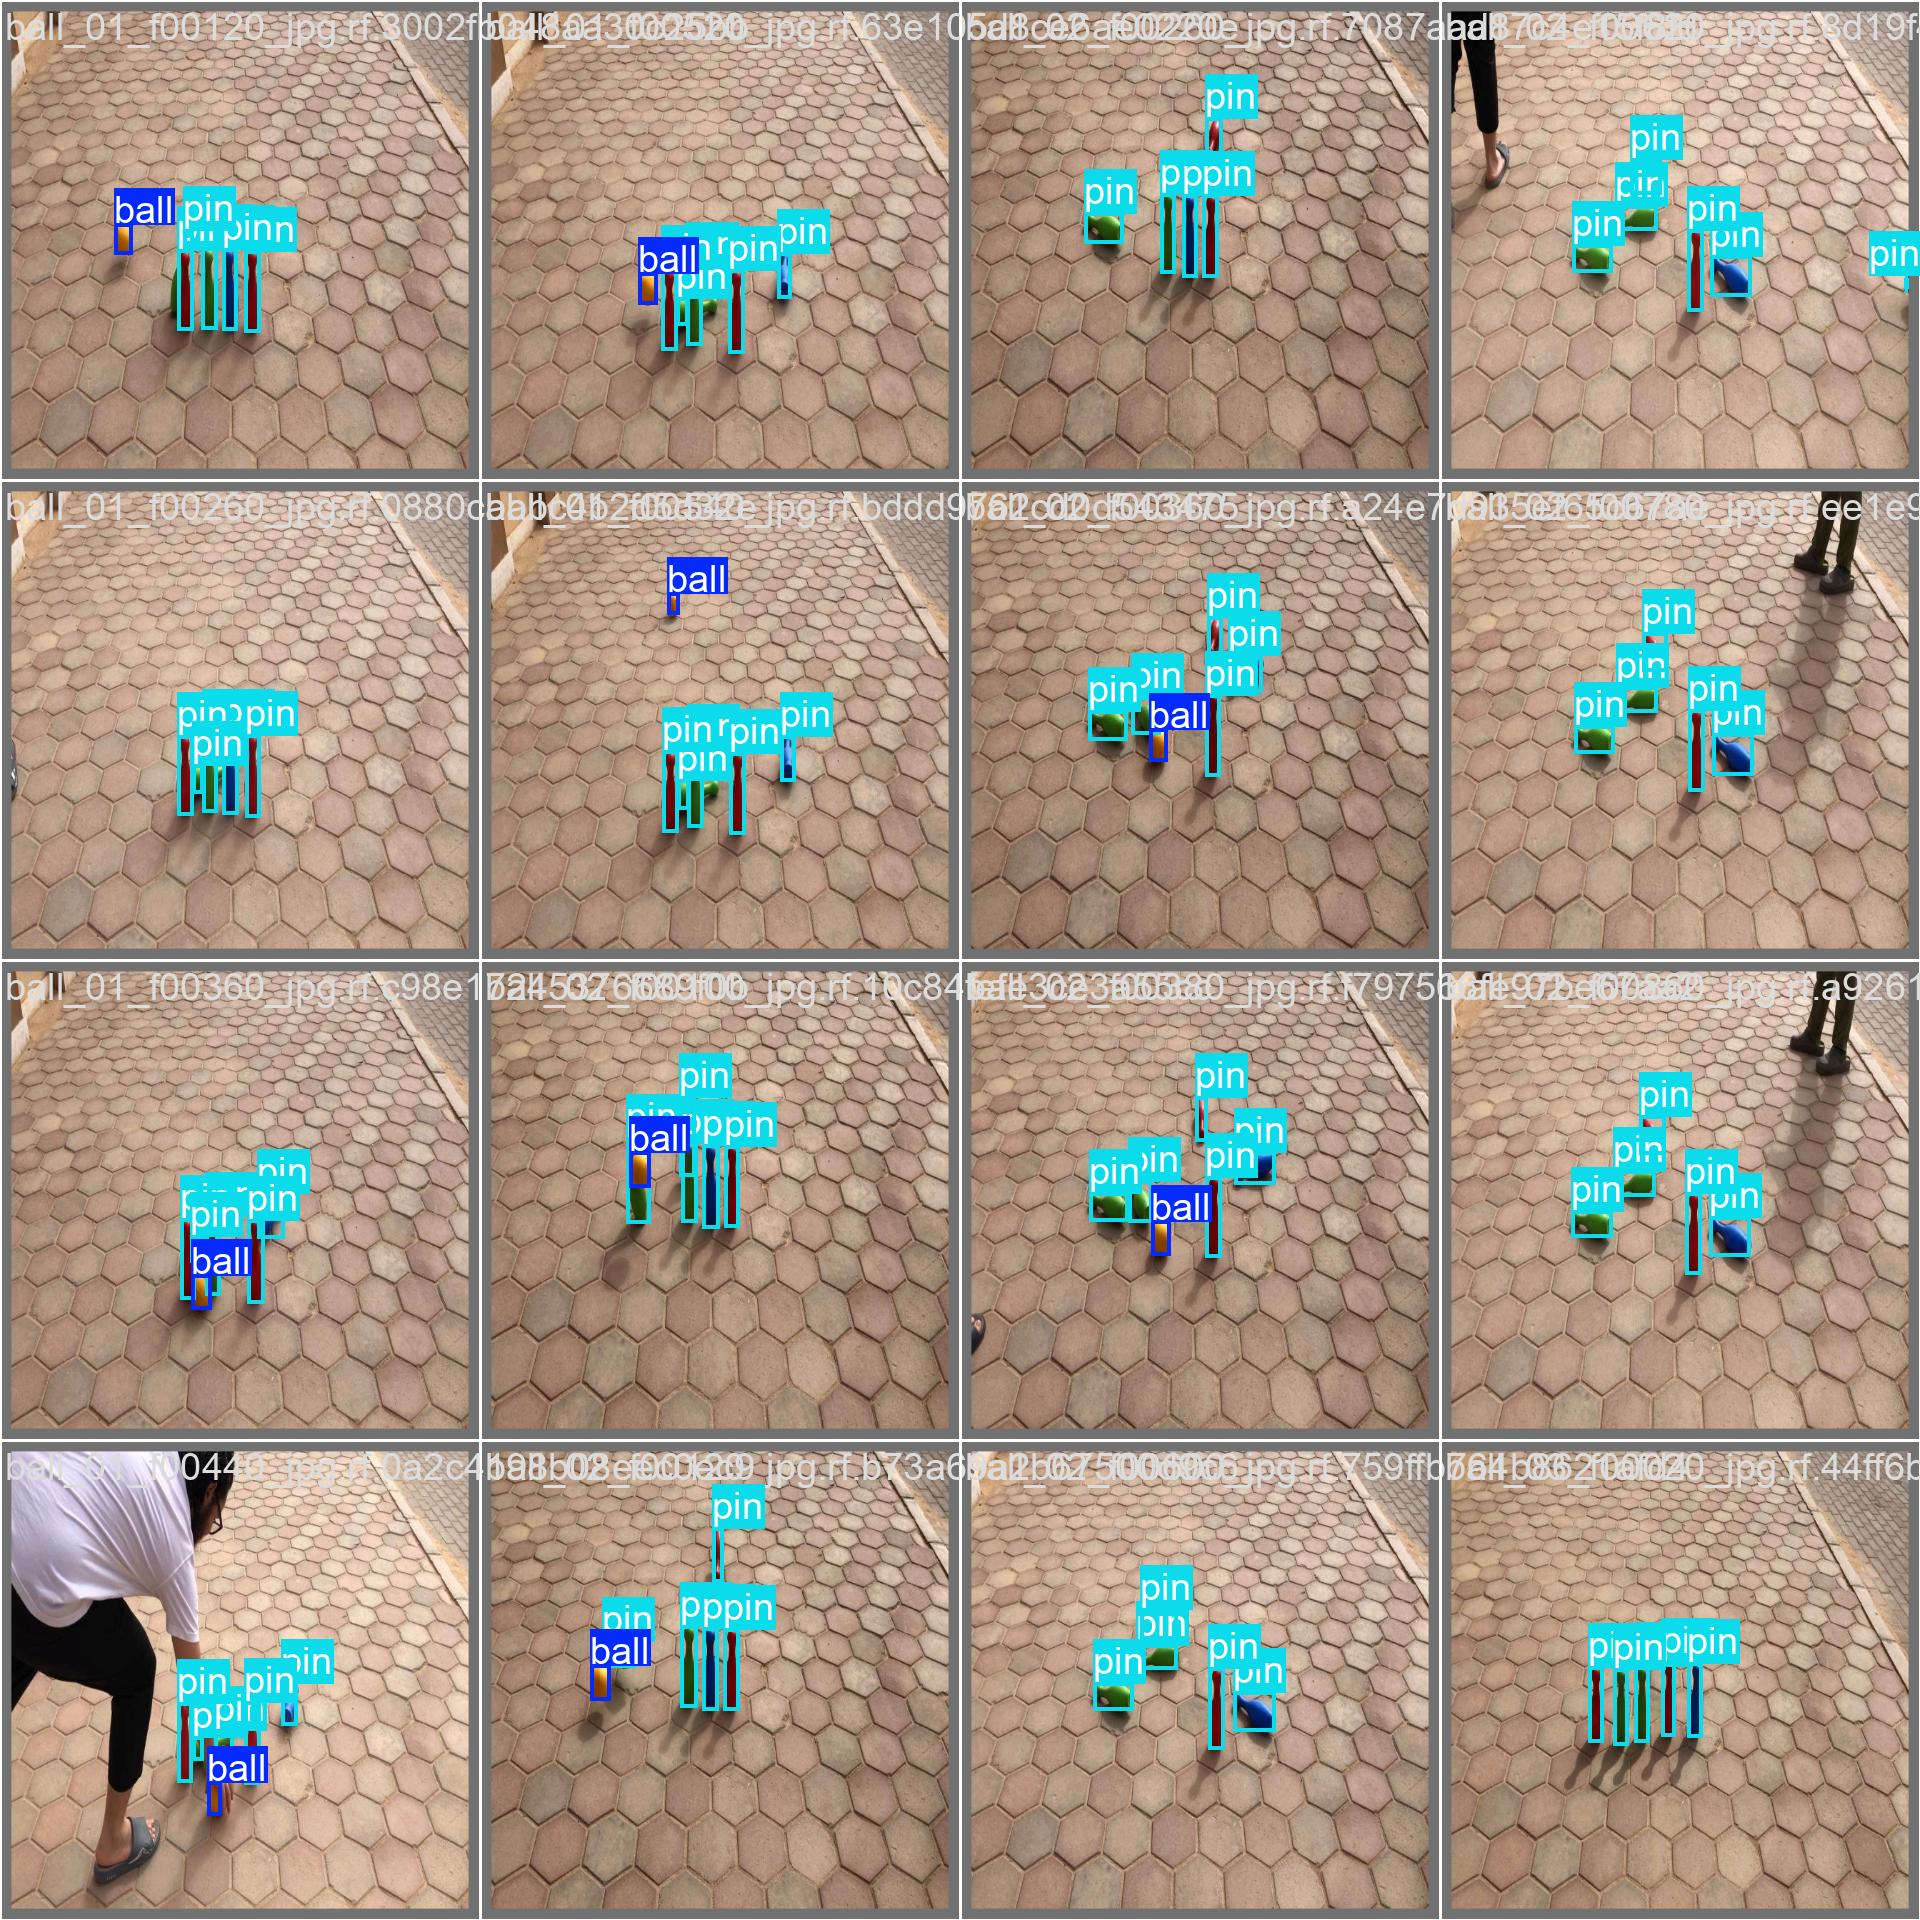
\includegraphics[width=\linewidth]{figures/val_batch0_labels.jpg}
      \small Example annotated frame
    \end{column}
  \end{columns}
\end{frame}

%% ============================================================
%% Slide 3 — System Pipeline
%% ============================================================
\begin{frame}{System Pipeline}
  \begin{enumerate}
    \item \textbf{Video Ingestion} --- OpenCV reads frames from MP4/MOV at original resolution and fps.
    \vspace{0.3em}
    \item \textbf{Detection} --- Fine-tuned YOLOv8s detects \texttt{ball} and \texttt{pin} in each frame (conf $= 0.10$). Ball boxes feed the proximity gate in Stage 4.
    \vspace{0.3em}
    \item \textbf{Tracking} --- ByteTrack assigns stable integer IDs to pin detections across frames, maintaining identity through brief occlusion.
    \vspace{0.3em}
    \item \textbf{Fall Determination} --- Per-ID 3-state machine (\textsc{Standing} $\to$ \textsc{Maybe\_Falling} $\to$ \textsc{Fallen}) uses aspect ratio and centroid-drop criteria, gated by ball proximity.
    \vspace{0.3em}
    \item \textbf{Rendering} --- OpenCV draws markers, timestamps, HUD, and final summary; \texttt{cv2.VideoWriter} encodes the output at original fps and resolution.
  \end{enumerate}
\end{frame}

%% ============================================================
%% Slide 4 — Dataset
%% ============================================================
\begin{frame}{Dataset}
  \begin{columns}[T]
    \begin{column}{0.52\textwidth}
      \textbf{Recording Protocol}
      \begin{itemize}
        \item 15 iPhone clips, $\approx$30 fps, MOV/H.264
        \item Same indoor environment, varied pin layouts (triangle, scattered, line)
        \item No controlled studio setup
      \end{itemize}
      \vspace{0.5em}
      \textbf{Frame Extraction}
      \begin{itemize}
        \item Stride 1:20 ($\approx$1.5 fps effective)
        \item Long edge resized to 1280 px (\texttt{INTER\_AREA})
        \item \textbf{557 keyframes} extracted total
      \end{itemize}
      \vspace{0.5em}
      \textbf{Split \& Class Counts}\\[0.3em]
      \small
      \begin{tabular}{lrr}
        \toprule
        Split & Frames & Ball / Pin \\
        \midrule
        Train & 407 & 162 / 2{,}291 \\
        Val   & 100 & --- \\
        Test  &  50 & --- \\
        \bottomrule
      \end{tabular}
    \end{column}
    \begin{column}{0.46\textwidth}
      \centering
      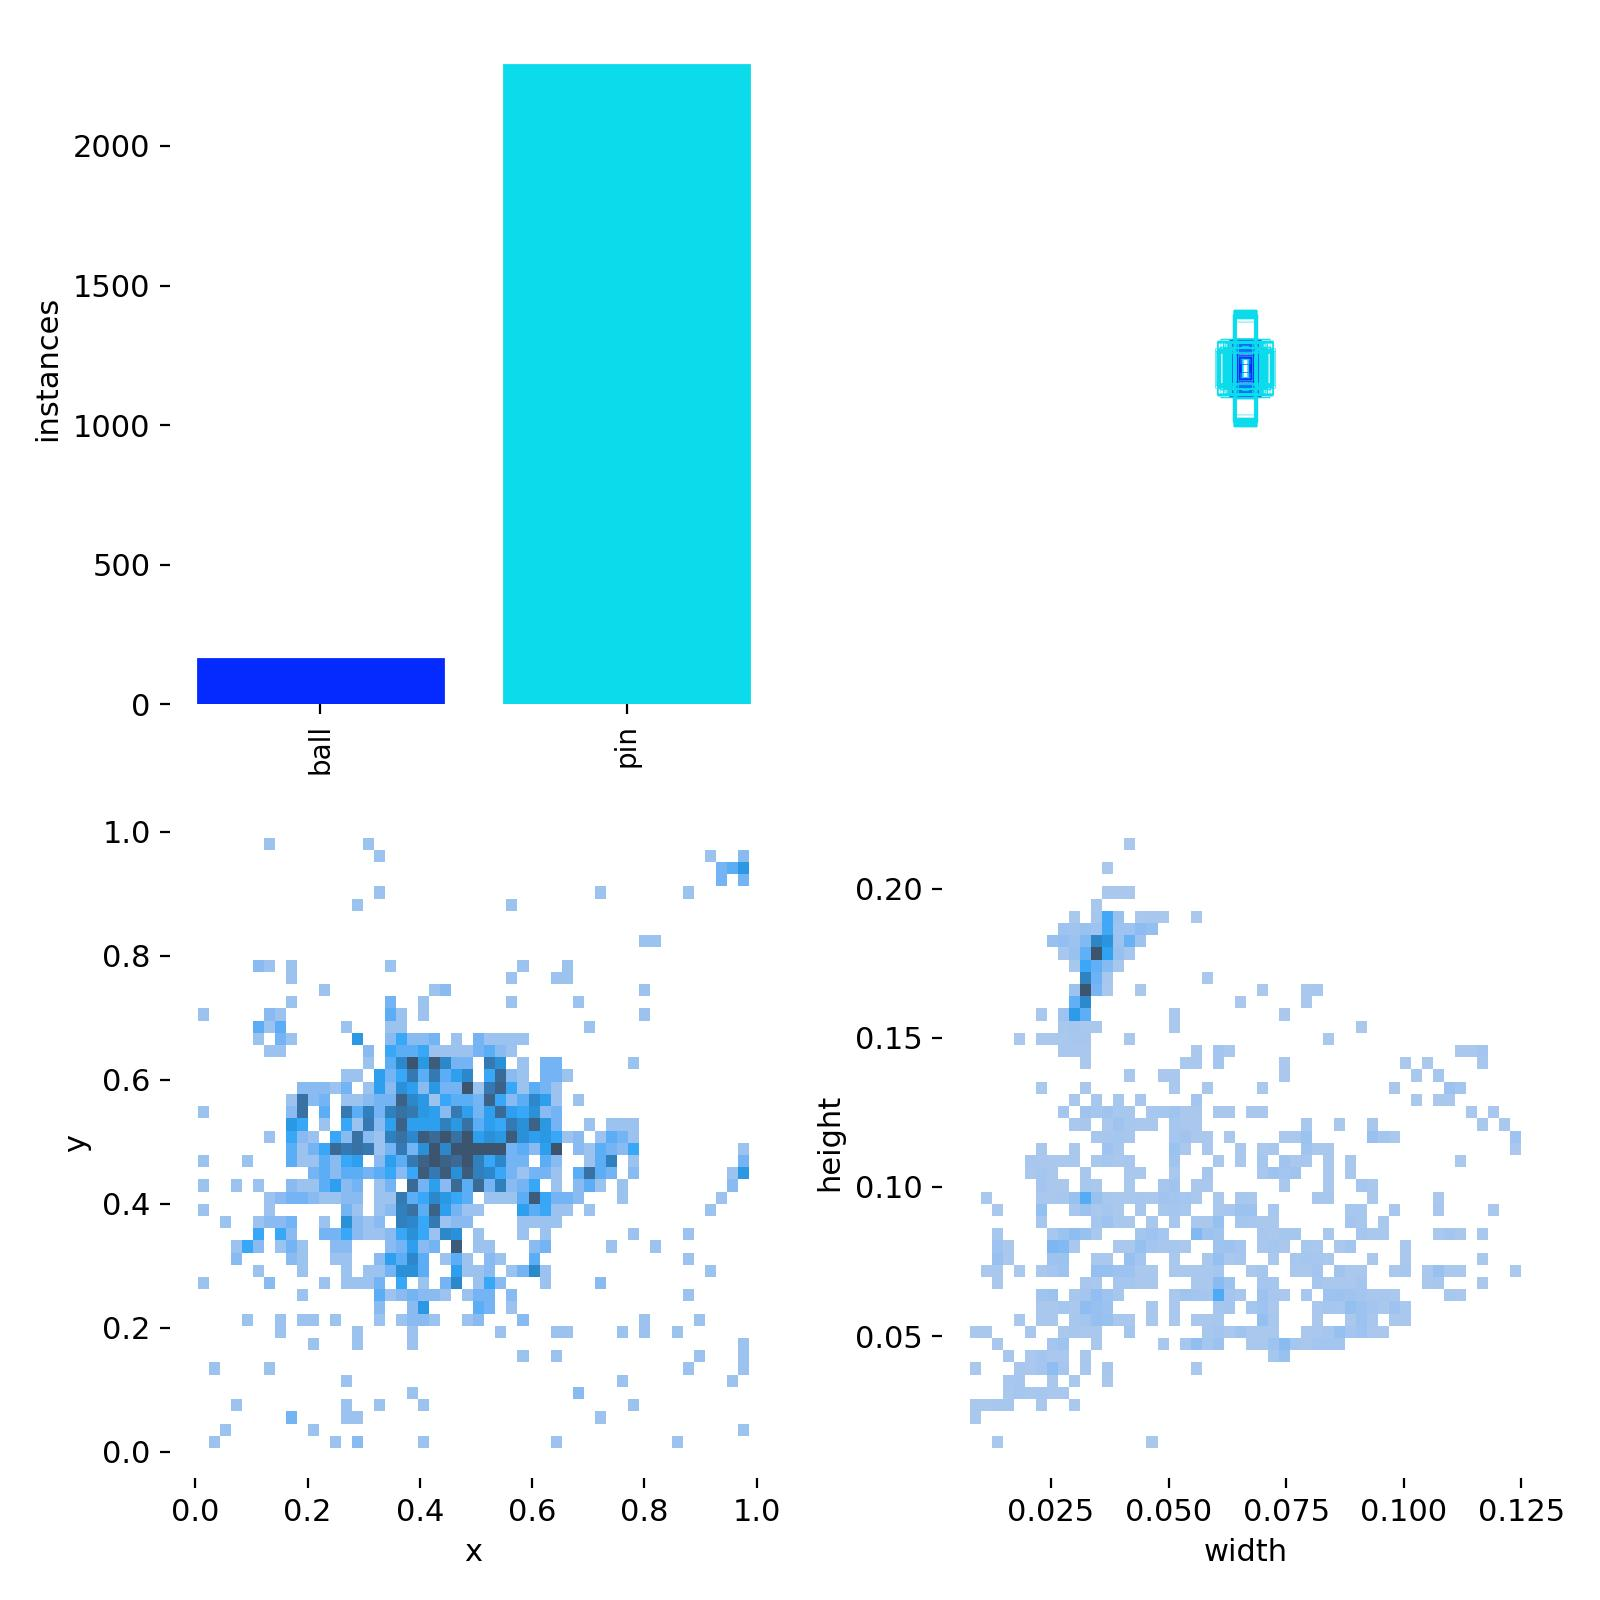
\includegraphics[width=\linewidth]{figures/labels.jpg}
      \small Training-set label distribution
    \end{column}
  \end{columns}
\end{frame}

%% ============================================================
%% Slide 5 — Data Remediation
%% ============================================================
\begin{frame}{Data Remediation}
  \begin{columns}[T]
    \begin{column}{0.55\textwidth}
      \textbf{Problem:} Roboflow exported \emph{polygon} labels, not axis-aligned bounding boxes.
      Training on the raw export caused \textbf{catastrophic convergence failure} (loss did not decrease, zero detections).
      \vspace{0.5em}

      \textbf{Three operations applied to 3,051 polygon annotations:}
      \begin{enumerate}
        \item \textbf{Polygon $\to$ bbox conversion} --- derive $x_{\min}, x_{\max}, y_{\min}, y_{\max}$ from polygon vertices; compute $x_c, y_c, w, h$.
        \item \textbf{Coordinate clamping} --- clamp all values to $[0, 1]$ to remove out-of-bounds vertices.
        \item \textbf{Extreme-box filtering} --- remove annotations with $w$ or $h > 0.45$ or $< 0.005$.
      \end{enumerate}

      \vspace{0.3em}
      After remediation training converged normally.
    \end{column}
    \begin{column}{0.42\textwidth}
      \centering
      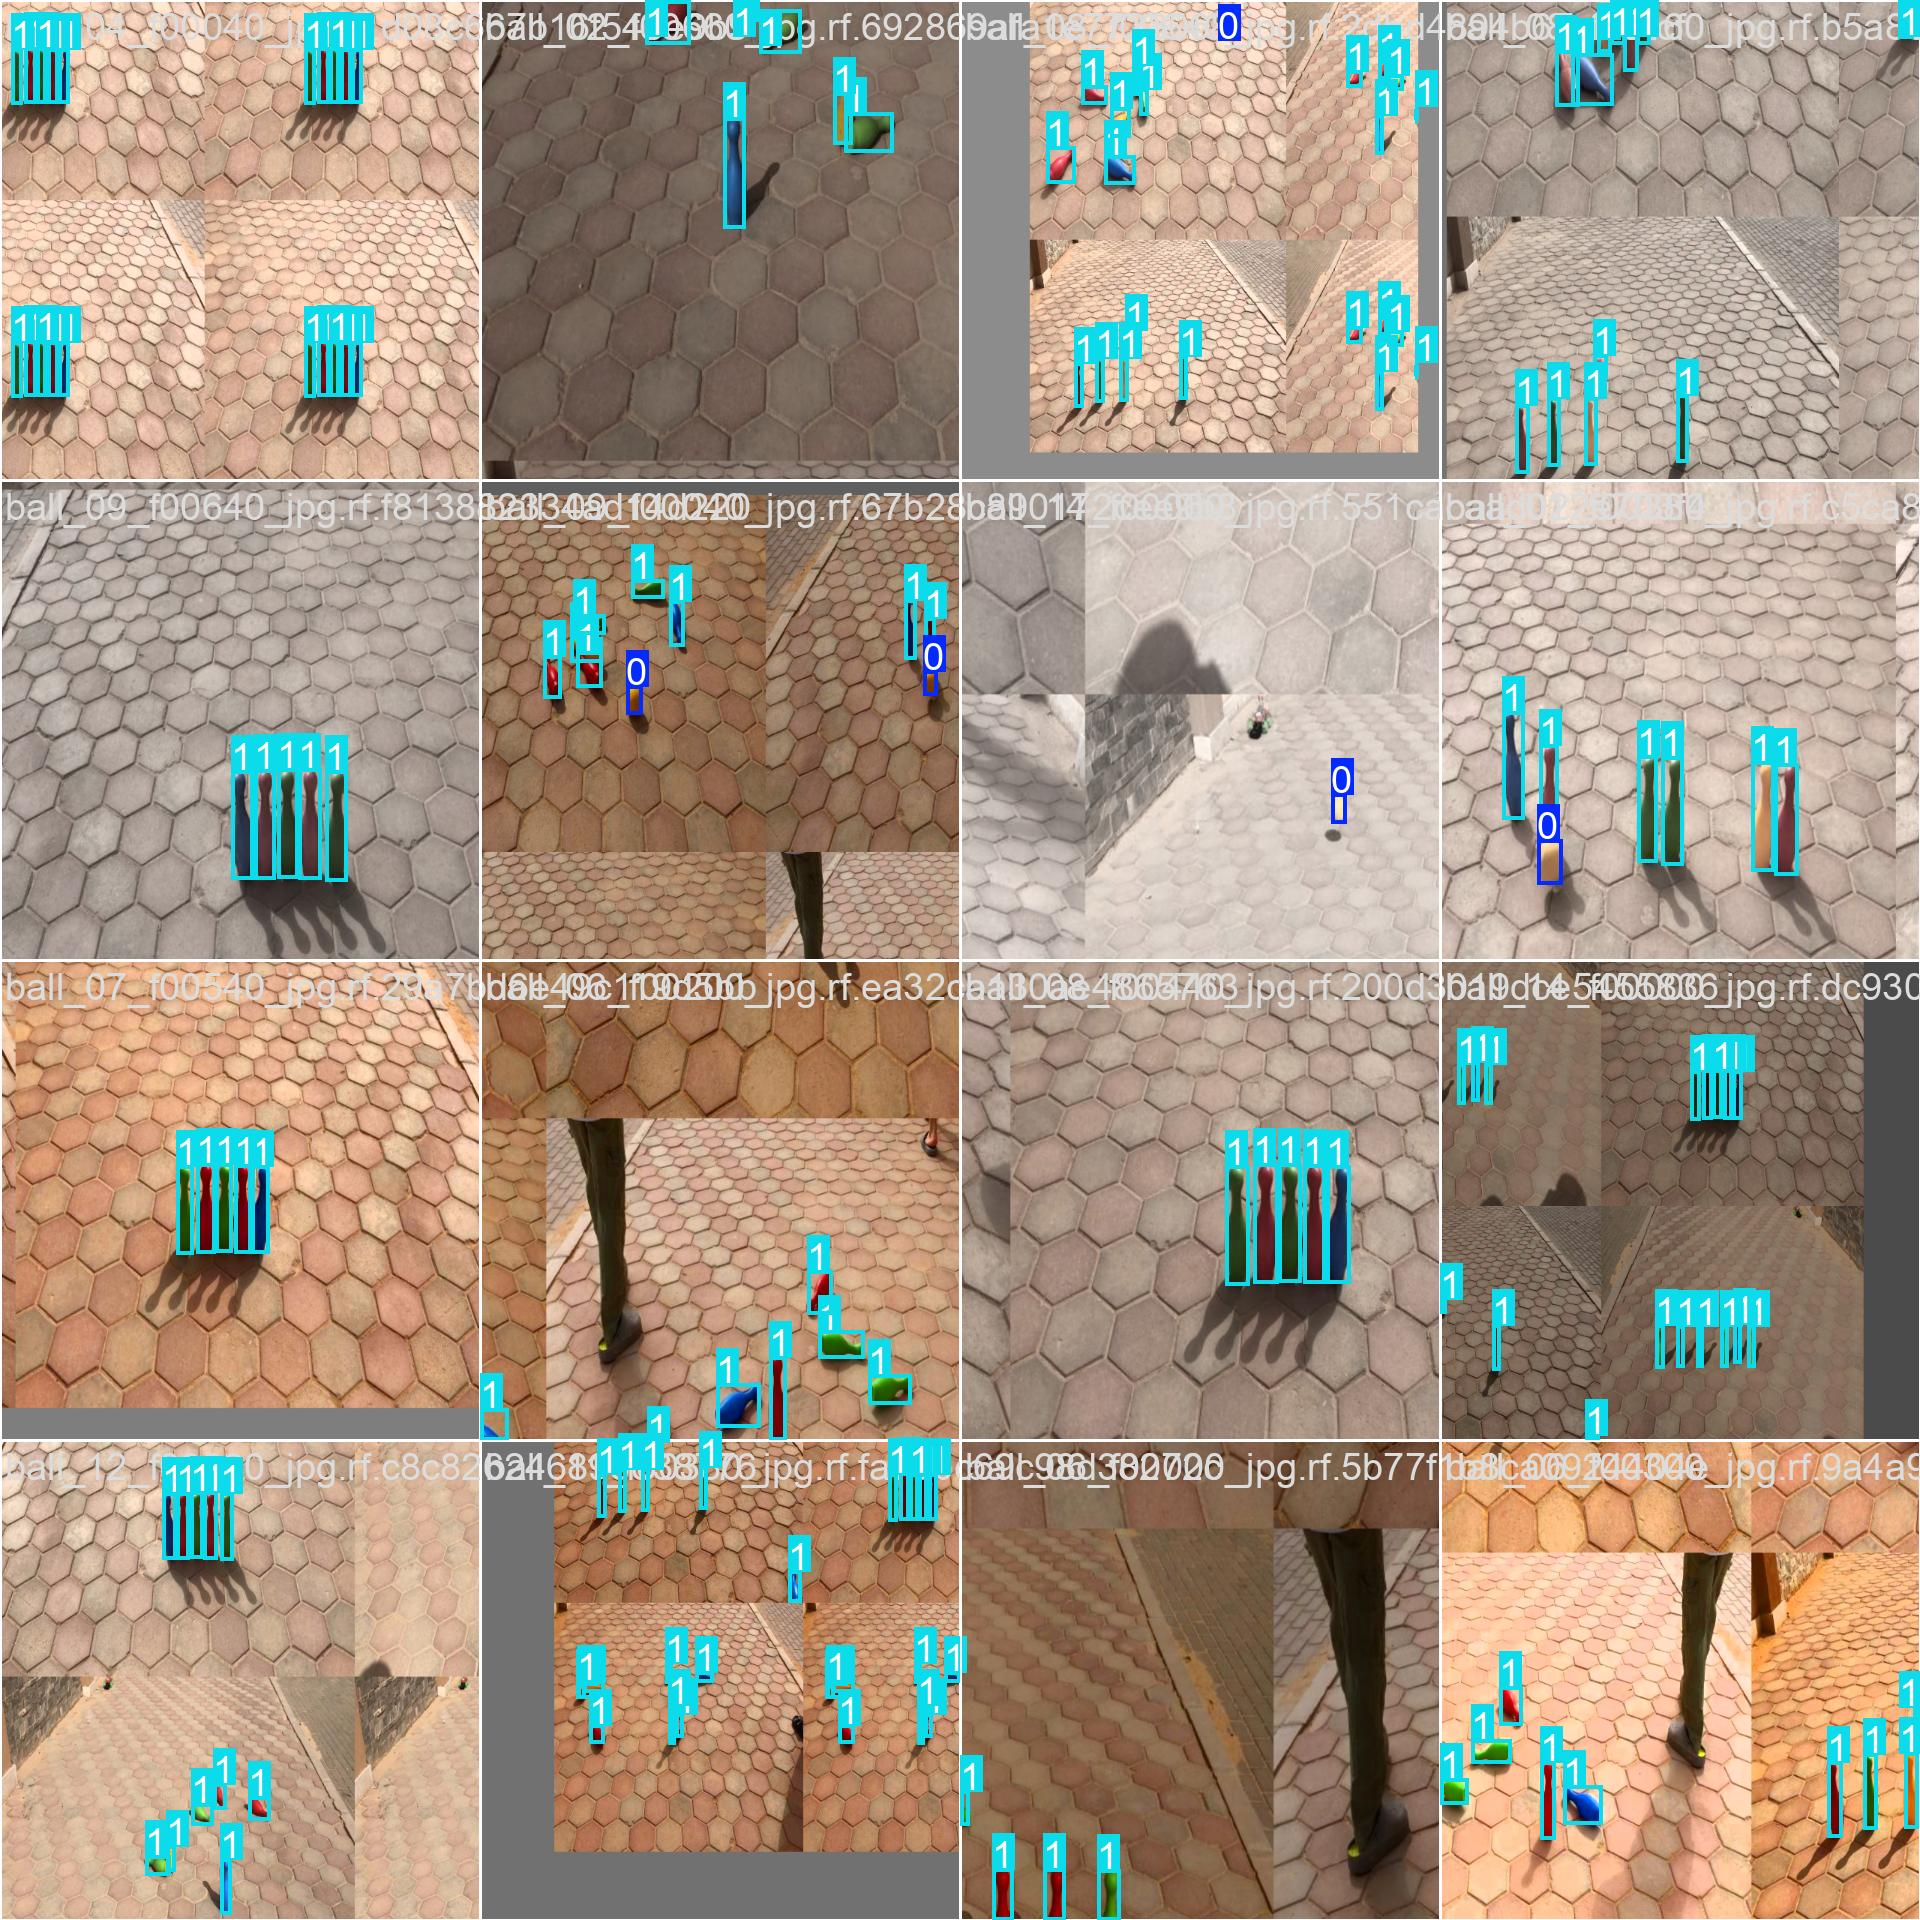
\includegraphics[width=\linewidth]{figures/train_batch0.jpg}
      \small Epoch 1 training batch --- correctly aligned boxes after remediation
    \end{column}
  \end{columns}
\end{frame}

%% ============================================================
%% Slide 6 — Model Selection: Why YOLOv8s
%% ============================================================
\begin{frame}{Model Selection: Why YOLOv8s}
  \begin{columns}[T]
    \begin{column}{0.55\textwidth}
      \small
      \begin{tabular}{lp{5.5cm}}
        \toprule
        Option & Assessment \\
        \midrule
        YOLOv8n & Misses small/distant pins; insufficient recall. \\
        \textbf{YOLOv8s} & \textbf{Chosen.} Good recall on small objects; fast training. \\
        YOLOv8m/l/x & Negligible gain on $\sim$700 images; $3$--$5\times$ longer training. \\
        Faster R-CNN & Higher ceiling in principle; heavy engineering overhead not justified by dataset size. \\
        Custom CNN & Strictly worse than a fine-tuned pretrained model at this scale. \\
        Classical CV & Brittle to lighting and orientation; does not satisfy the modelling requirement. \\
        \bottomrule
      \end{tabular}
      \vspace{0.5em}

      \textbf{Key facts:} YOLOv8s, 11M parameters, pretrained on COCO,
      fine-tuned on our 2-class dataset.
    \end{column}
    \begin{column}{0.42\textwidth}
      \centering
      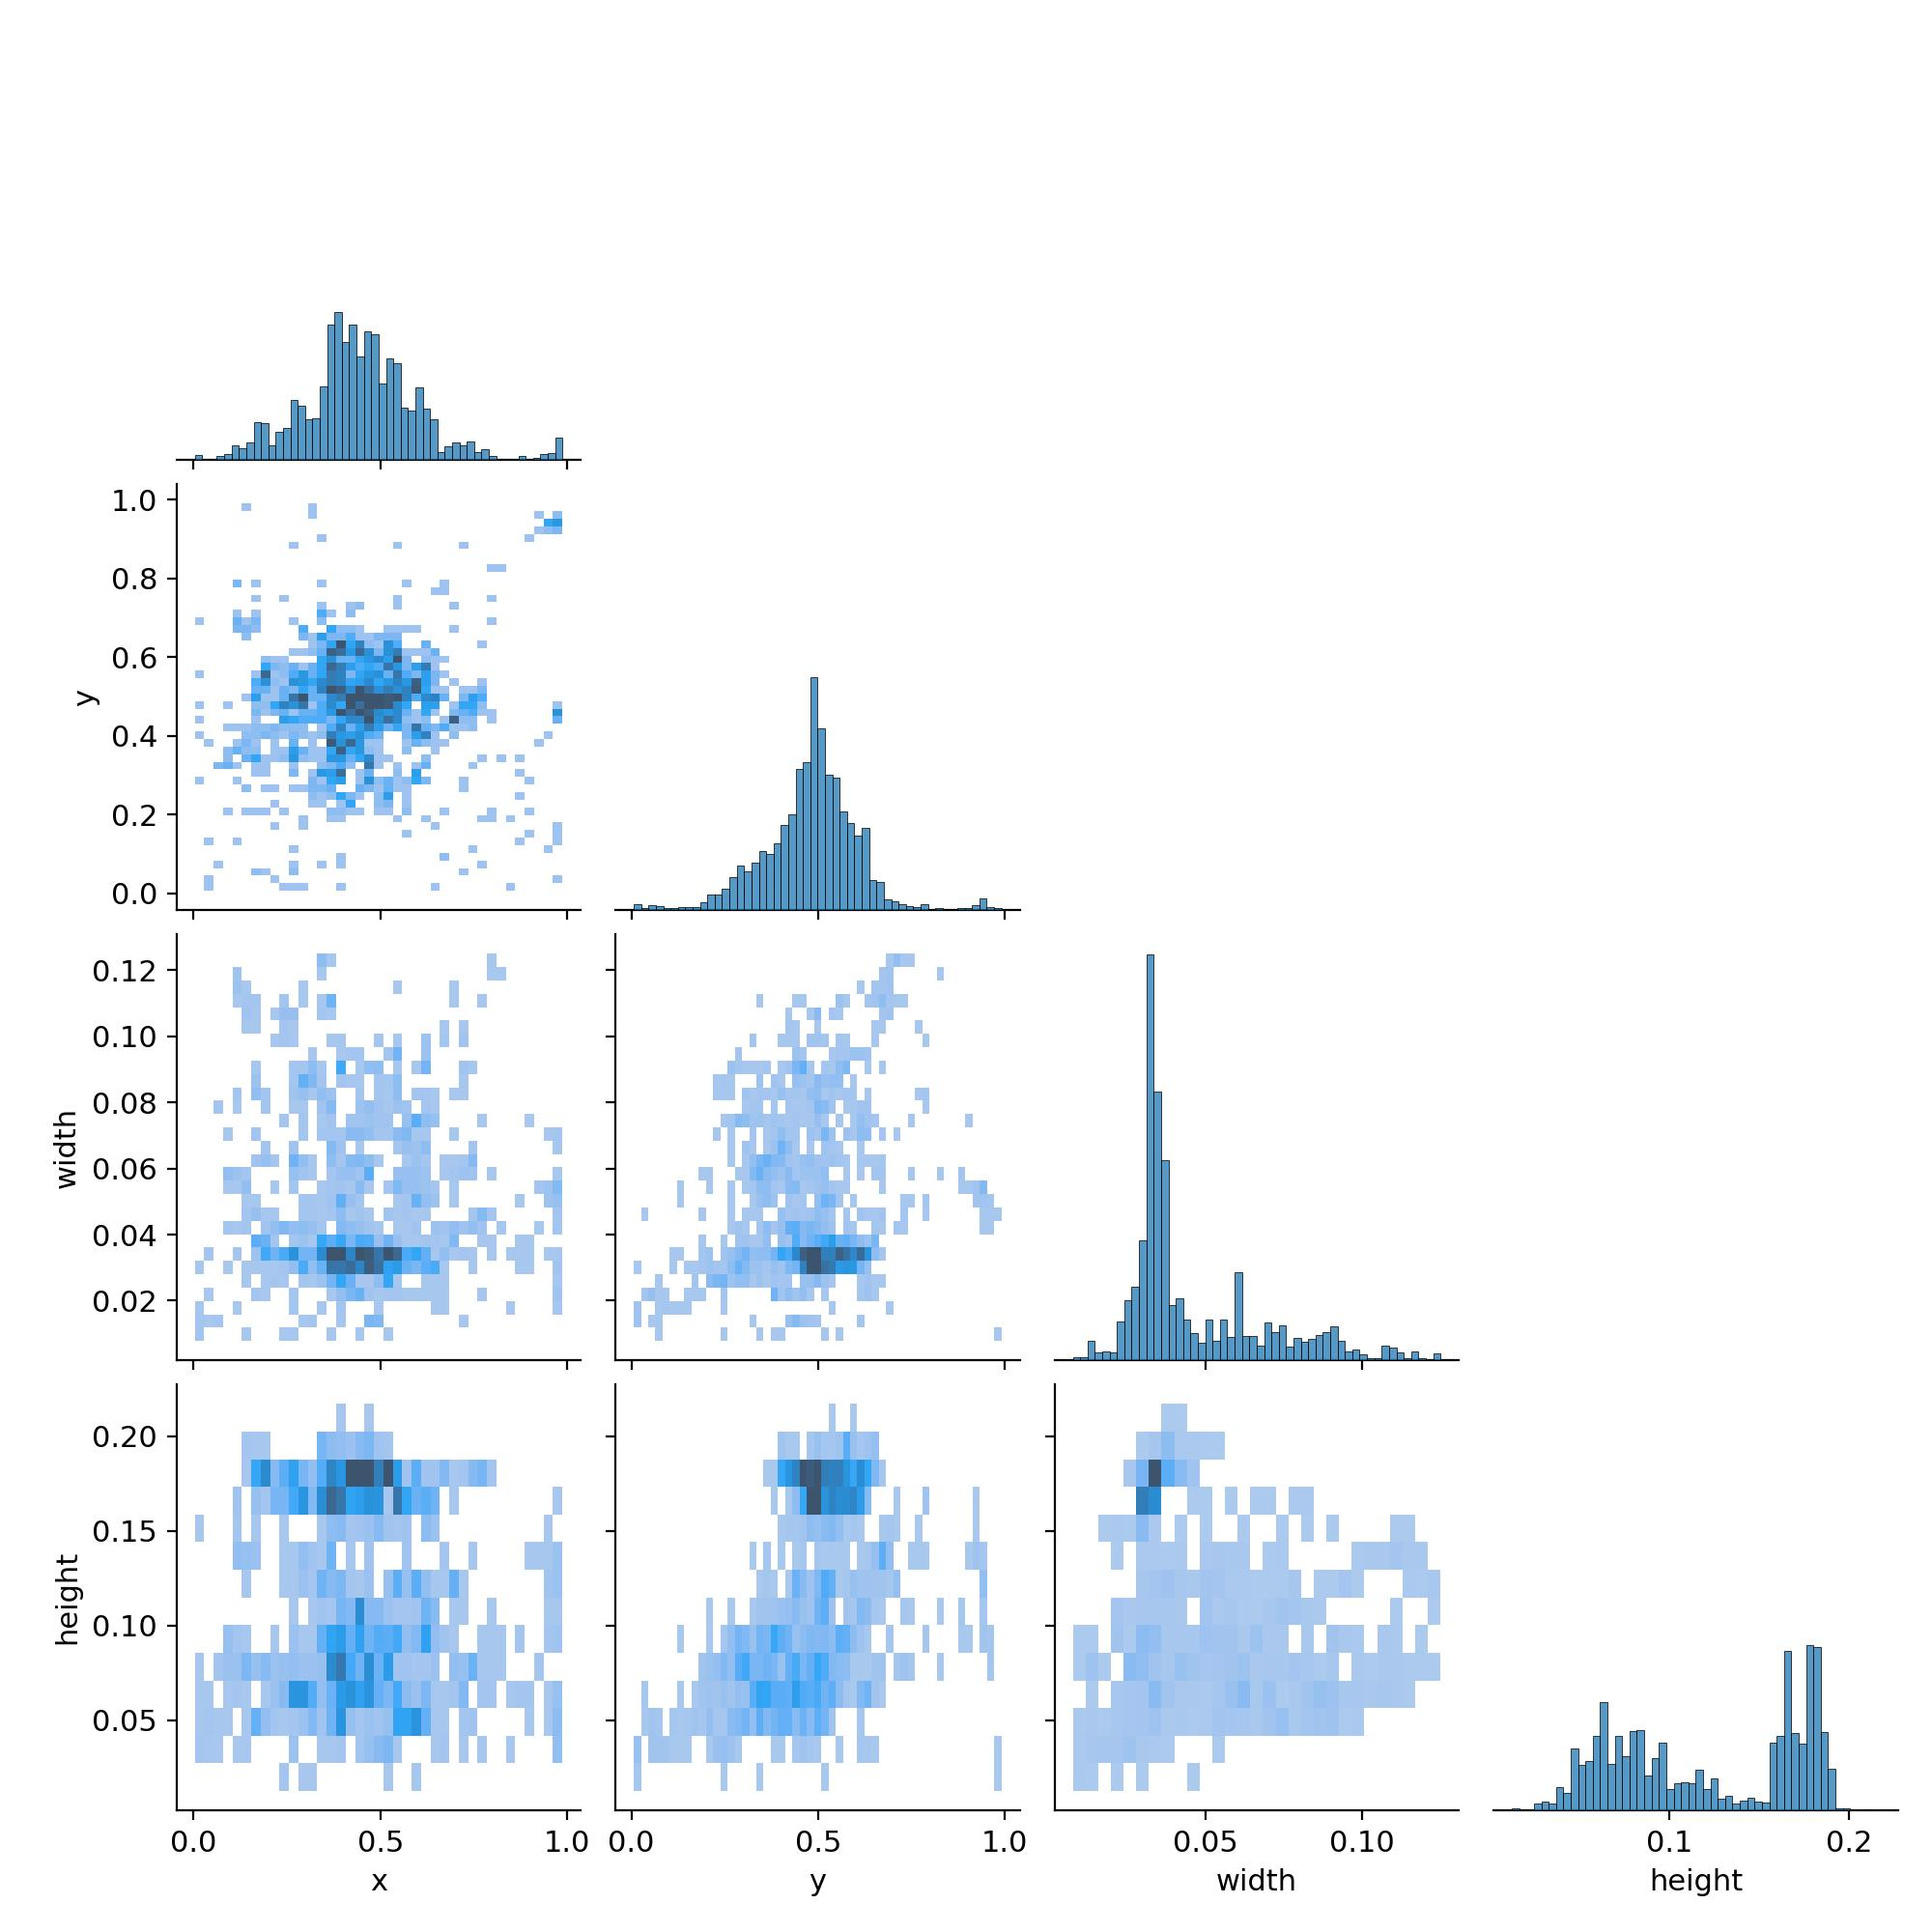
\includegraphics[width=\linewidth]{figures/labels_correlogram.jpg}
      \small Label spatial distribution (training set)
    \end{column}
  \end{columns}
\end{frame}

%% ============================================================
%% Slide 7 — Why One Class for Pins
%% ============================================================
\begin{frame}{Why One Class for Pins}
  \textbf{Intuitive design:} Two classes --- \texttt{standing\_pin} and \texttt{fallen\_pin}.
  Class output would directly indicate fall state. \textbf{This was rejected.}

  \vspace{0.8em}
  \textbf{The problem with two pin classes:}
  \begin{itemize}
    \item ByteTrack maintains a stable ID by matching detections across frames using IoU and appearance.
    \item When a pin falls, its bounding box changes shape substantially: tall and narrow $\to$ wide and short.
    \item If the \emph{class label also changes} at that same frame, ByteTrack sees a disappearing \texttt{standing\_pin} and a new \texttt{fallen\_pin} --- and assigns a \textbf{new track ID}.
    \item The ID switch happens at exactly the frame where the fall event must be recorded under the \emph{original} ID.
    \item The state machine would never see the transition on a consistent identity.
  \end{itemize}

  \vspace{0.5em}
  \textbf{Solution:} Single \texttt{pin} class. The tracker matches through the shape change via IoU, preserving the ID. Fall detection is done geometrically on the stable ID.
\end{frame}

%% ============================================================
%% Slide 8 — Fall Detection: State Machine
%% ============================================================
\begin{frame}{Fall Detection: State Machine}
  \textbf{Why single-frame detection fails:} perspective (axial falls), motion blur ($2$--$3$ frames), occlusion during impact.

  \vspace{0.5em}
  \textbf{3-State machine per track ID:}
  \[
    \textsc{Standing}
    \;\xrightarrow{\text{criterion met}}\;
    \textsc{Maybe\_Falling}
    \;\xrightarrow{\text{sustained 5 consecutive frames}}\;
    \textsc{Fallen}
  \]
  If criterion fails in \textsc{Maybe\_Falling}, counter resets $\to$ back to \textsc{Standing}.

  \vspace{0.5em}
  \textbf{Fall criterion (either condition is sufficient):}
  \[
    \frac{h}{w} < 0.9 \quad\textbf{OR}\quad \Delta y_c > 0.5 \times h_0
  \]
  ($h/w$ = current aspect ratio; $\Delta y_c$ = centroid drop; $h_0$ = standing box height)

  \vspace{0.5em}
  \textbf{Ball-proximity gate:} fall can only \emph{begin} if the ball was within $2 \times h_{\mathrm{pin}}$ of the pin centroid in the last 60 frames. Prevents false positives from camera shake or background motion.
\end{frame}

%% ============================================================
%% Slide 9 — Training Configuration
%% ============================================================
\begin{frame}{Training Configuration}
  \begin{columns}[T]
    \begin{column}{0.42\textwidth}
      \centering
      \begin{tabular}{ll}
        \toprule
        Parameter & Value \\
        \midrule
        Model      & YOLOv8s \\
        Epochs     & 100 \\
        Batch      & 16 \\
        imgsz      & 640 \\
        Patience   & 20 \\
        lr0        & 0.01 \\
        cos\_lr    & True \\
        Optimizer  & auto \\
        Seed       & 42 \\
        Hardware   & Kaggle T4 GPU \\
        \bottomrule
      \end{tabular}
      \vspace{0.5em}

      \small Cosine LR reduces the learning rate smoothly, avoiding abrupt gradient steps that step-LR causes. Early stopping fires if val mAP does not improve for 20 epochs.
    \end{column}
    \begin{column}{0.55\textwidth}
      \centering
      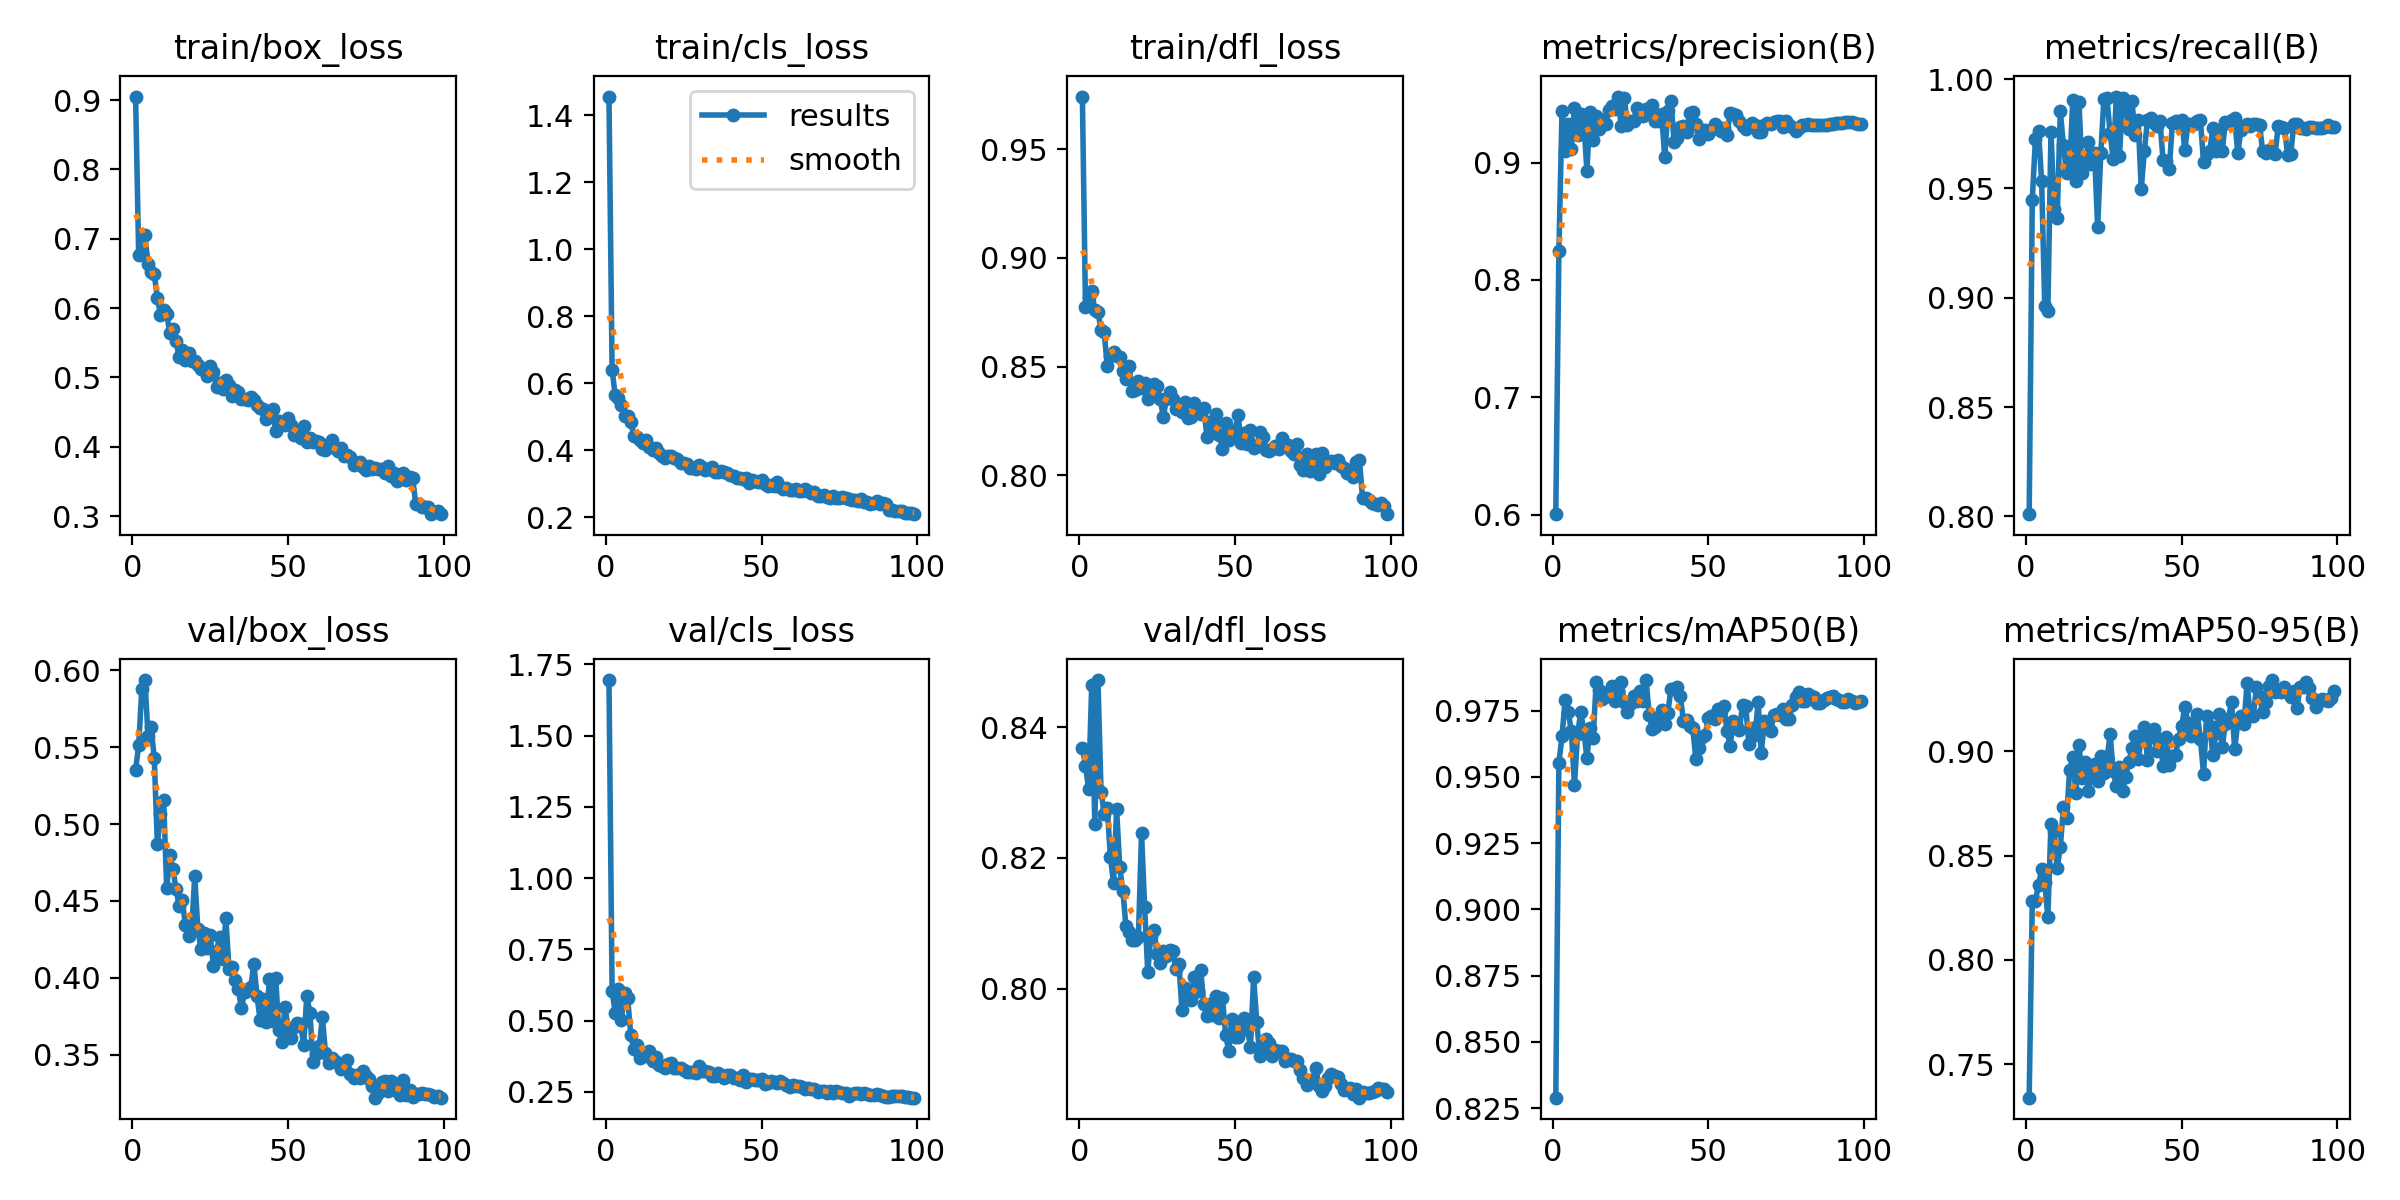
\includegraphics[width=\linewidth]{figures/results.png}
      \small Training convergence: losses and mAP across 100 epochs
    \end{column}
  \end{columns}
\end{frame}

%% ============================================================
%% Slide 10 — Quantitative Results
%% ============================================================
\begin{frame}{Quantitative Results}
  \begin{columns}[T]
    \begin{column}{0.50\textwidth}
      \small
      \begin{tabular}{lrr}
        \toprule
        Metric & Val & Test \\
        \midrule
        mAP@50       & 98.19\% & 97.19\% \\
        mAP@50-95    & 93.83\% & 91.21\% \\
        Precision    & 92.97\% & 97.69\% \\
        Recall       & 96.64\% & 88.59\% \\
        Max F1       & 0.9477  & ---     \\
        \midrule
        Ball AP@50   & 97.0\%  & ---     \\
        Pin AP@50    & 99.4\%  & ---     \\
        \bottomrule
      \end{tabular}
      \vspace{0.5em}

      Confidence threshold = 0.10 (F1 flat from 0.10 to 0.30; chosen for maximum recall).

      \vspace{0.3em}
      Test set used exactly once after all design decisions were frozen.
    \end{column}
    \begin{column}{0.48\textwidth}
      \centering
      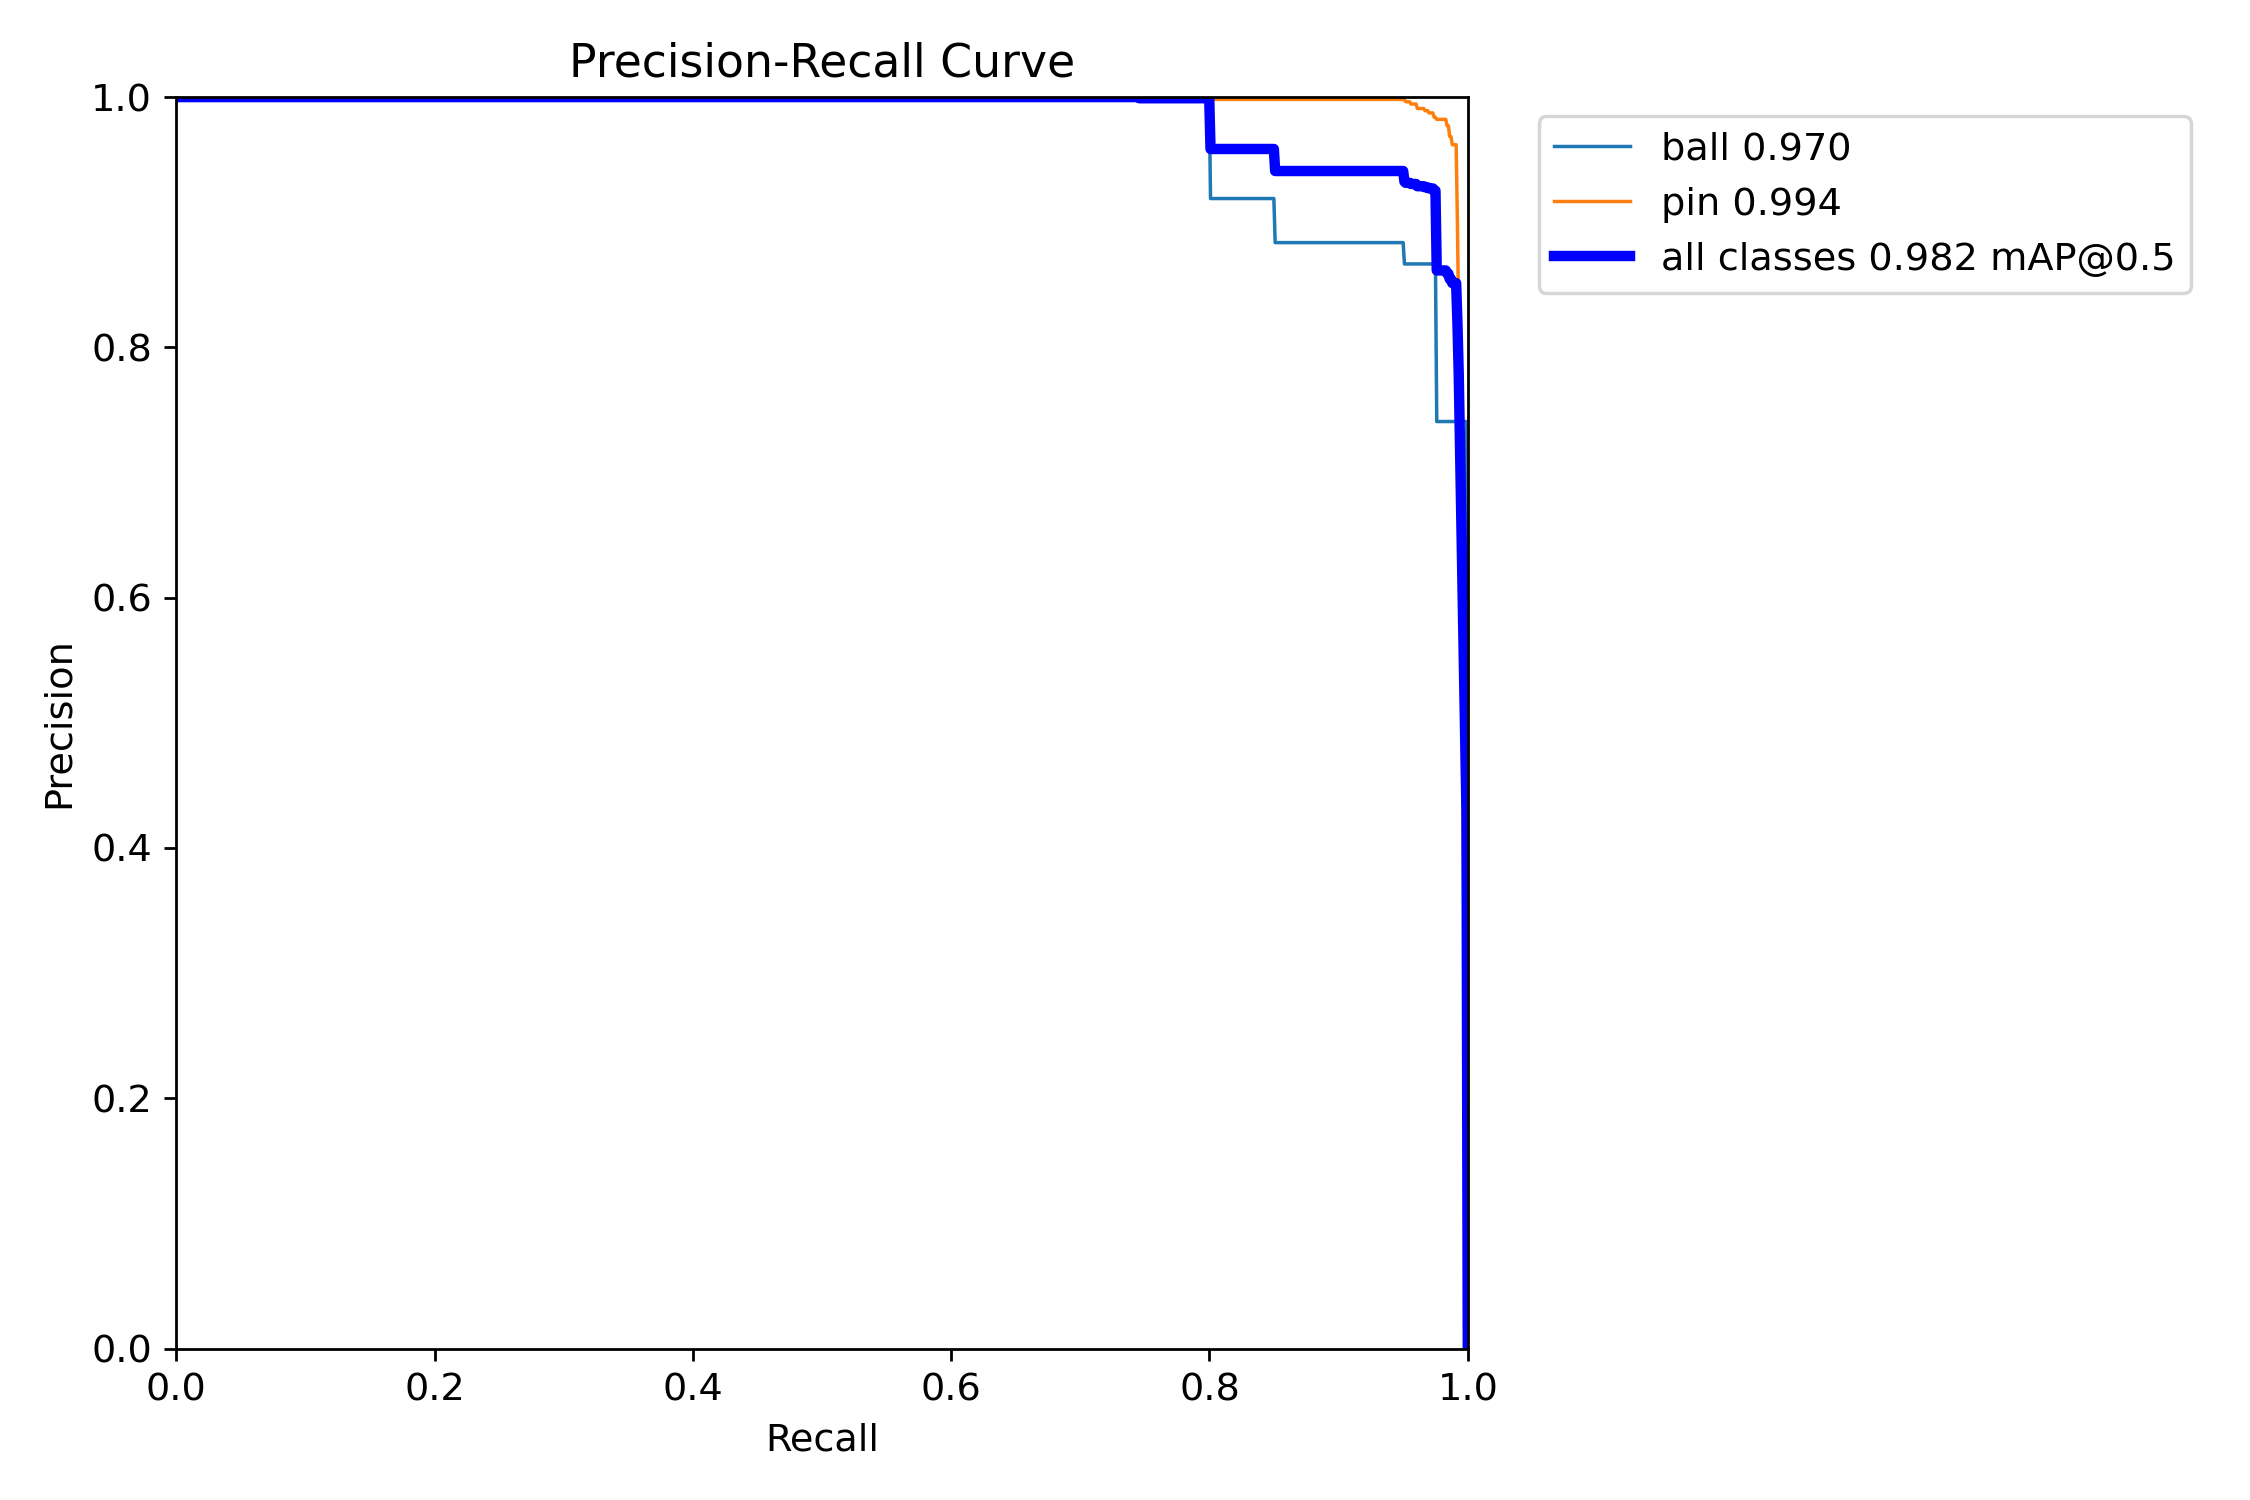
\includegraphics[width=\linewidth]{figures/PR_curve.png}
      \small Precision-Recall curve (validation set)
    \end{column}
  \end{columns}
\end{frame}

%% ============================================================
%% Slide 11 — Visual Diagnostics
%% ============================================================
\begin{frame}{Visual Diagnostics}
  \begin{columns}[T]
    \begin{column}{0.49\textwidth}
      \centering
      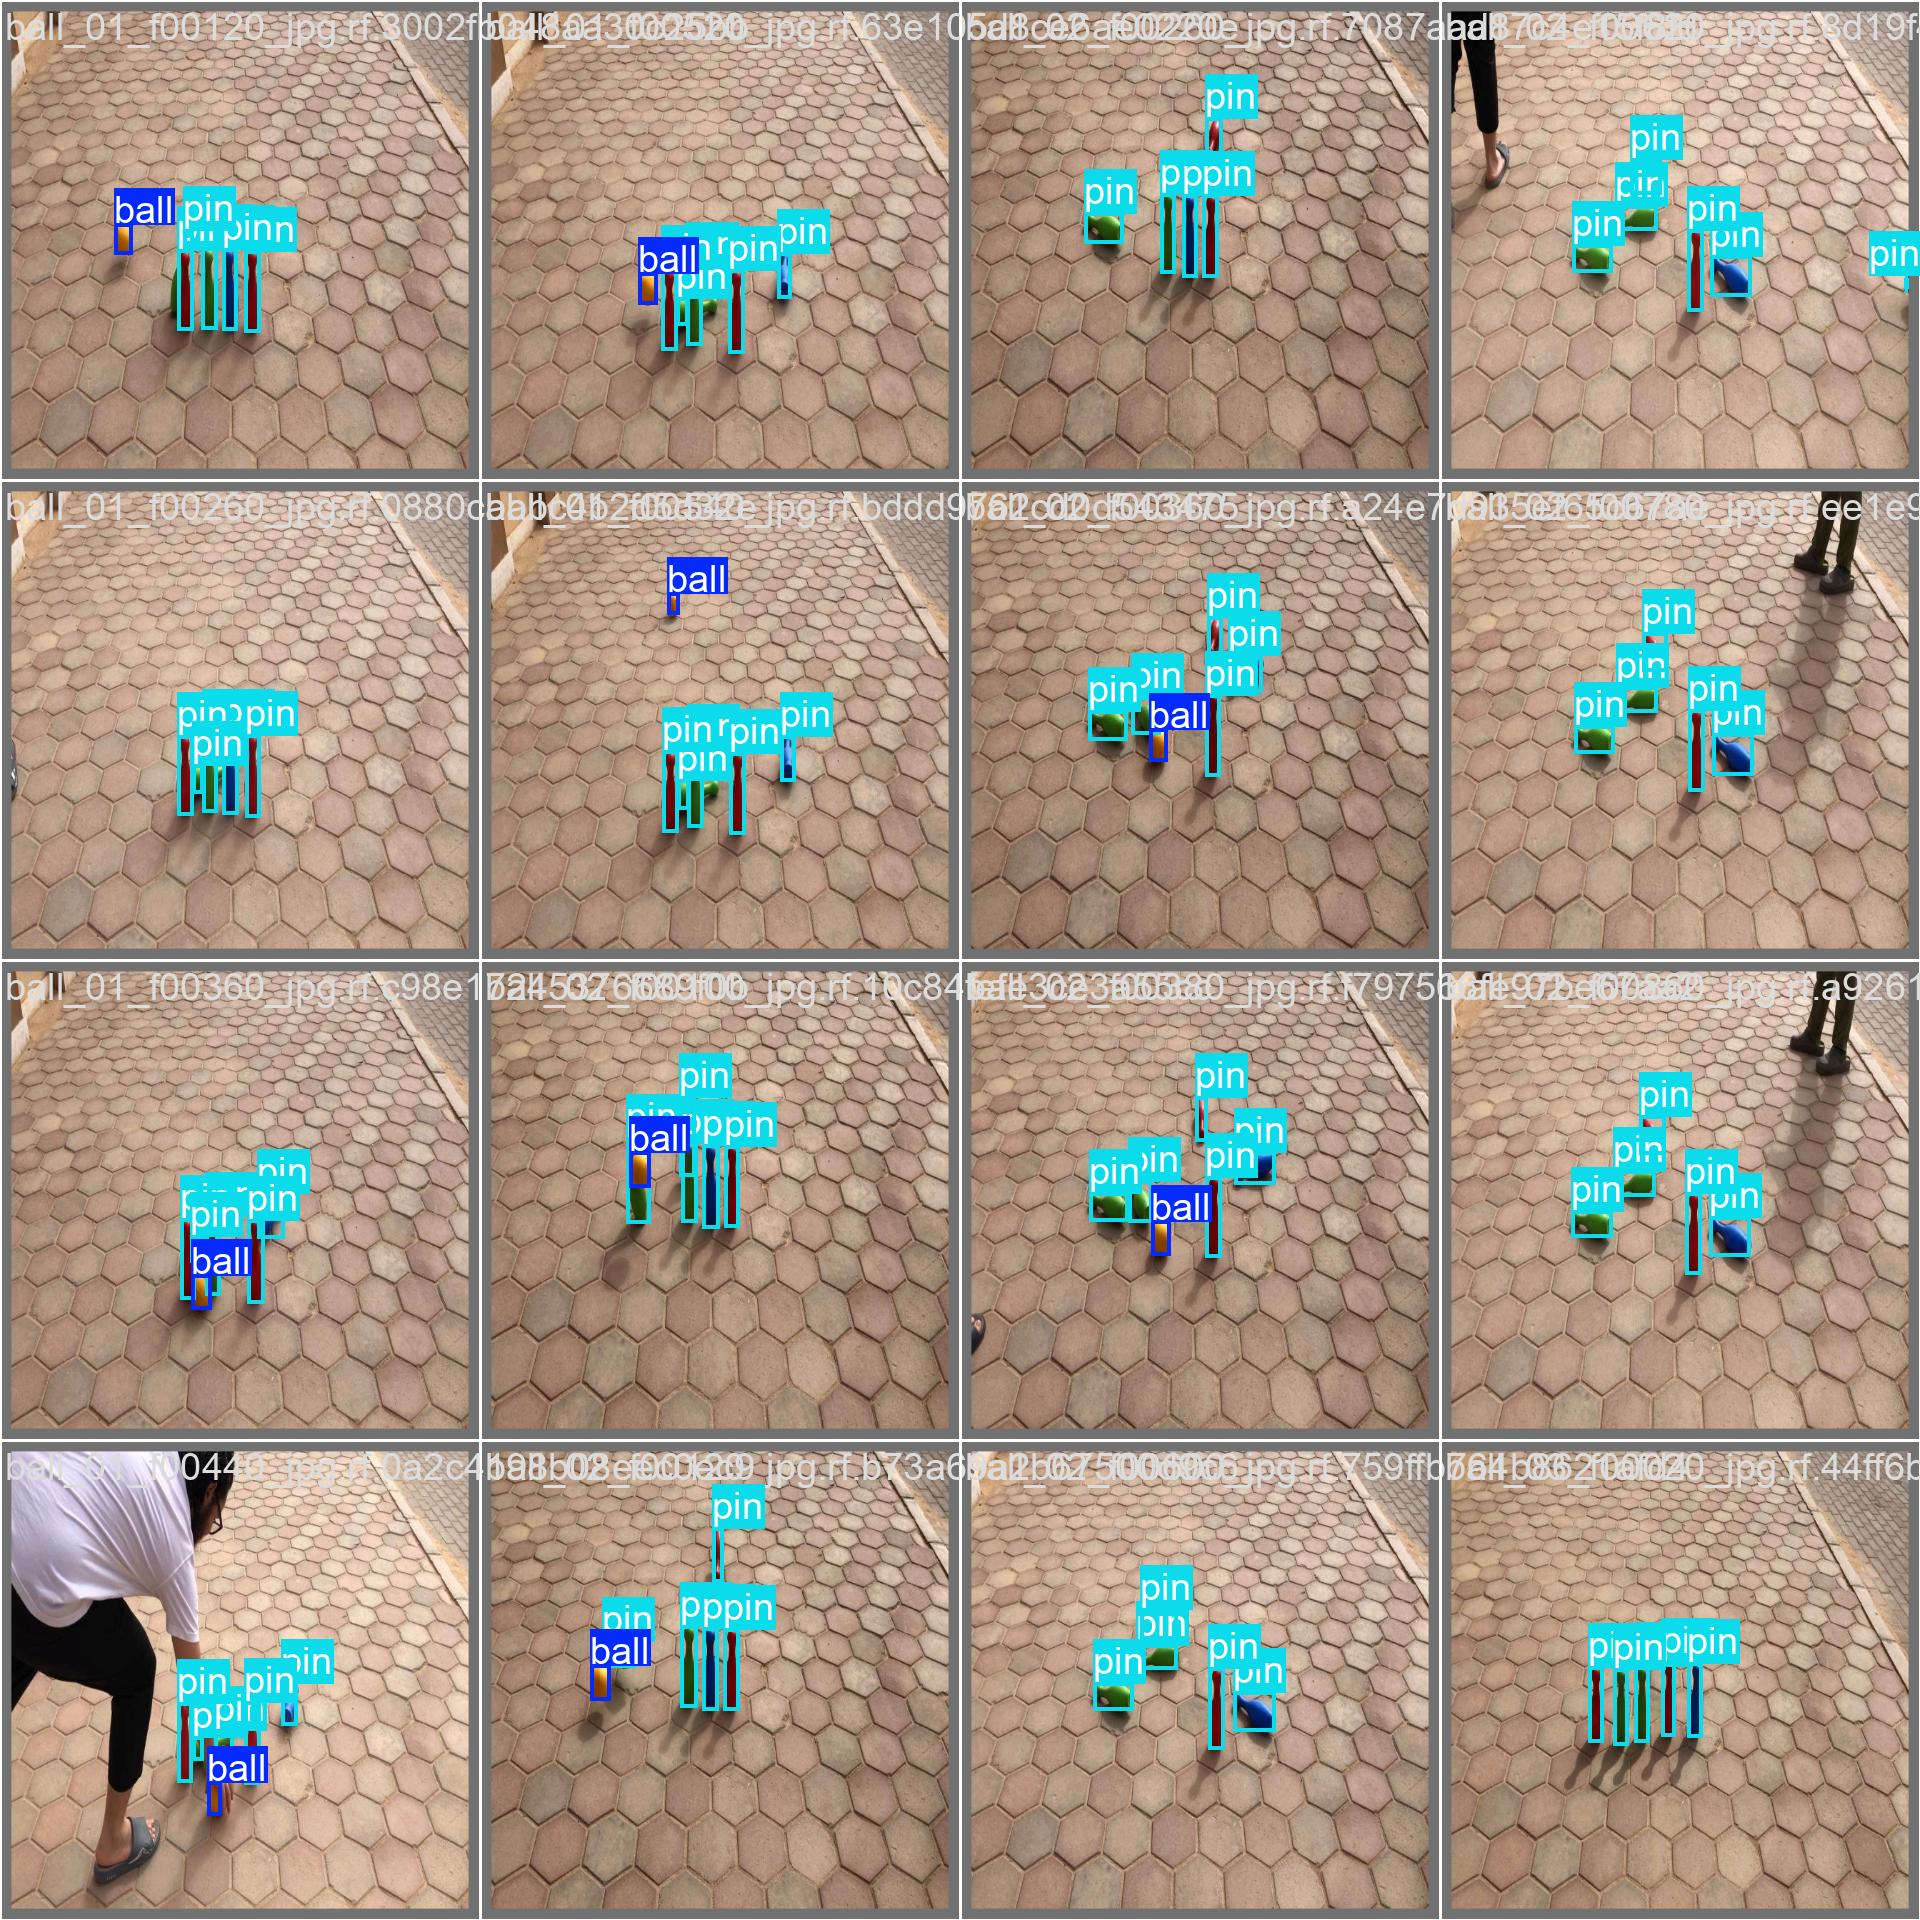
\includegraphics[width=\linewidth]{figures/val_batch0_labels.jpg}
      \small Ground truth labels (val batch 0)
    \end{column}
    \begin{column}{0.49\textwidth}
      \centering
      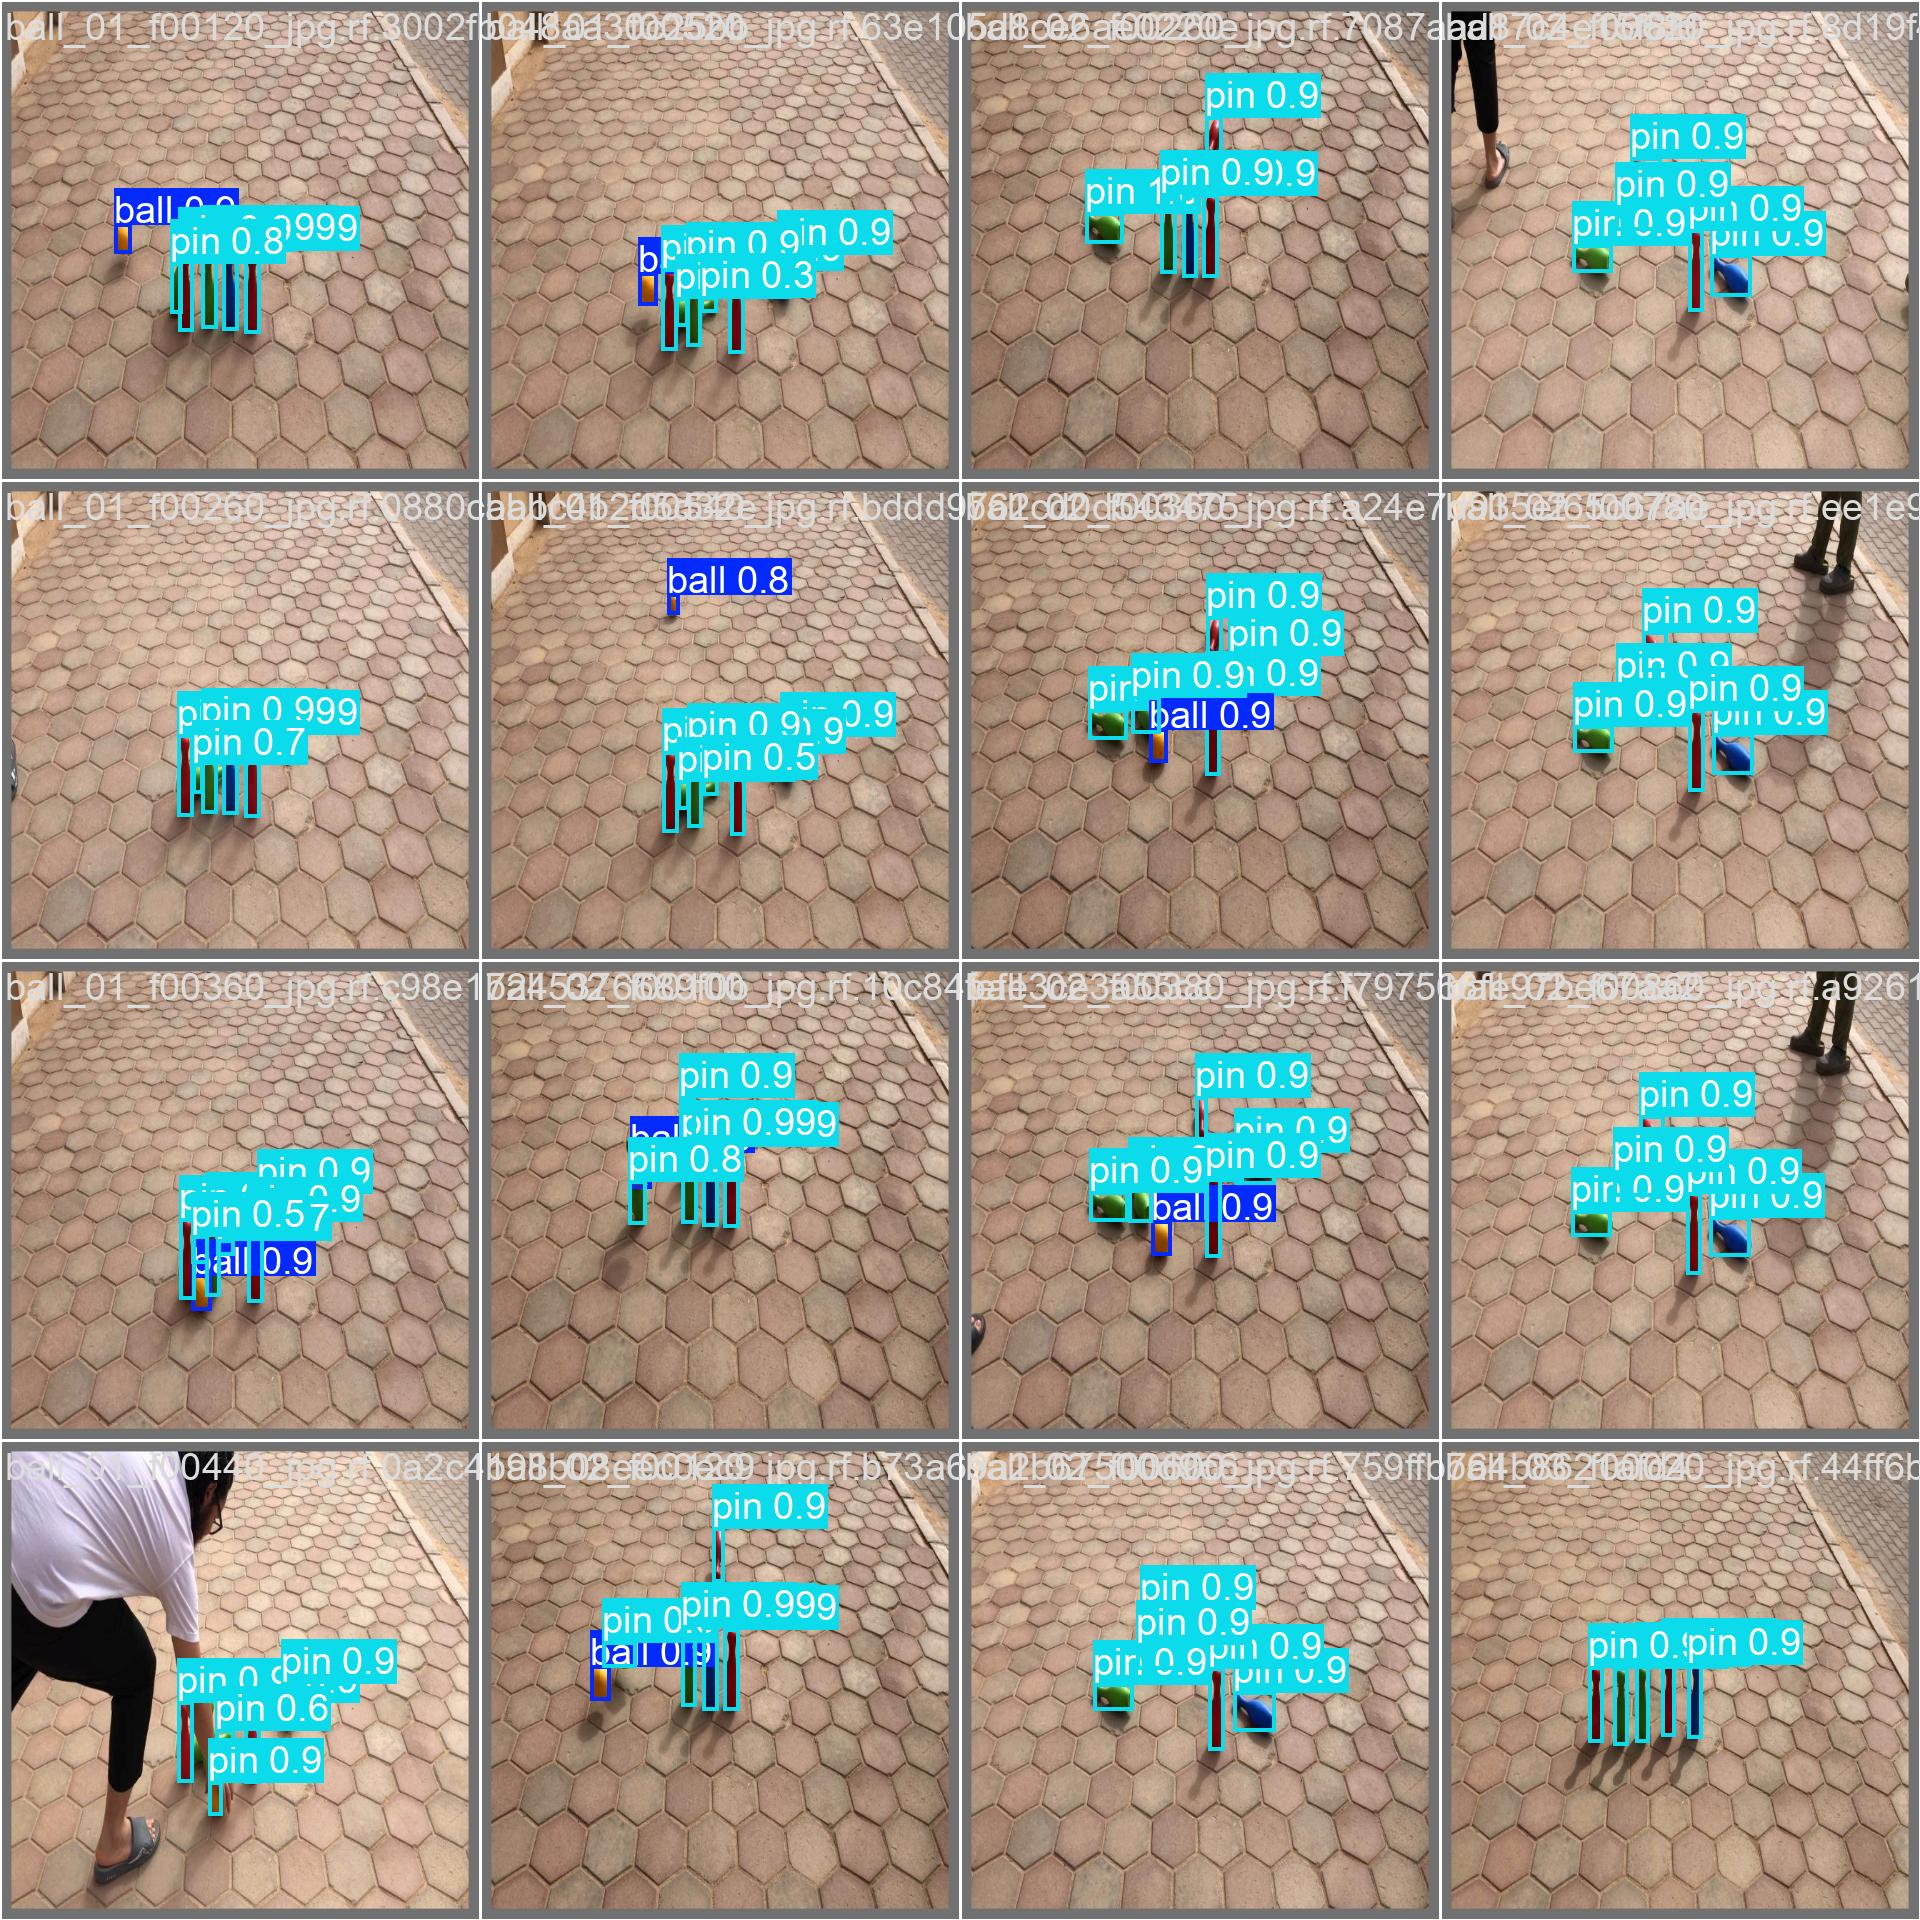
\includegraphics[width=\linewidth]{figures/val_batch0_pred.jpg}
      \small Model predictions (val batch 0)
    \end{column}
  \end{columns}
  \vspace{0.4em}
  \centering
  \small Predicted boxes are tightly aligned with ground truth across both ball and pin detections. Missed detections are rare; most occur on heavily occluded or motion-blurred instances.
\end{frame}

%% ============================================================
%% Slide 12 — Confusion Matrix + F1 Curve
%% ============================================================
\begin{frame}{Confusion Matrix \& F1 Curve}
  \begin{columns}[T]
    \begin{column}{0.49\textwidth}
      \centering
      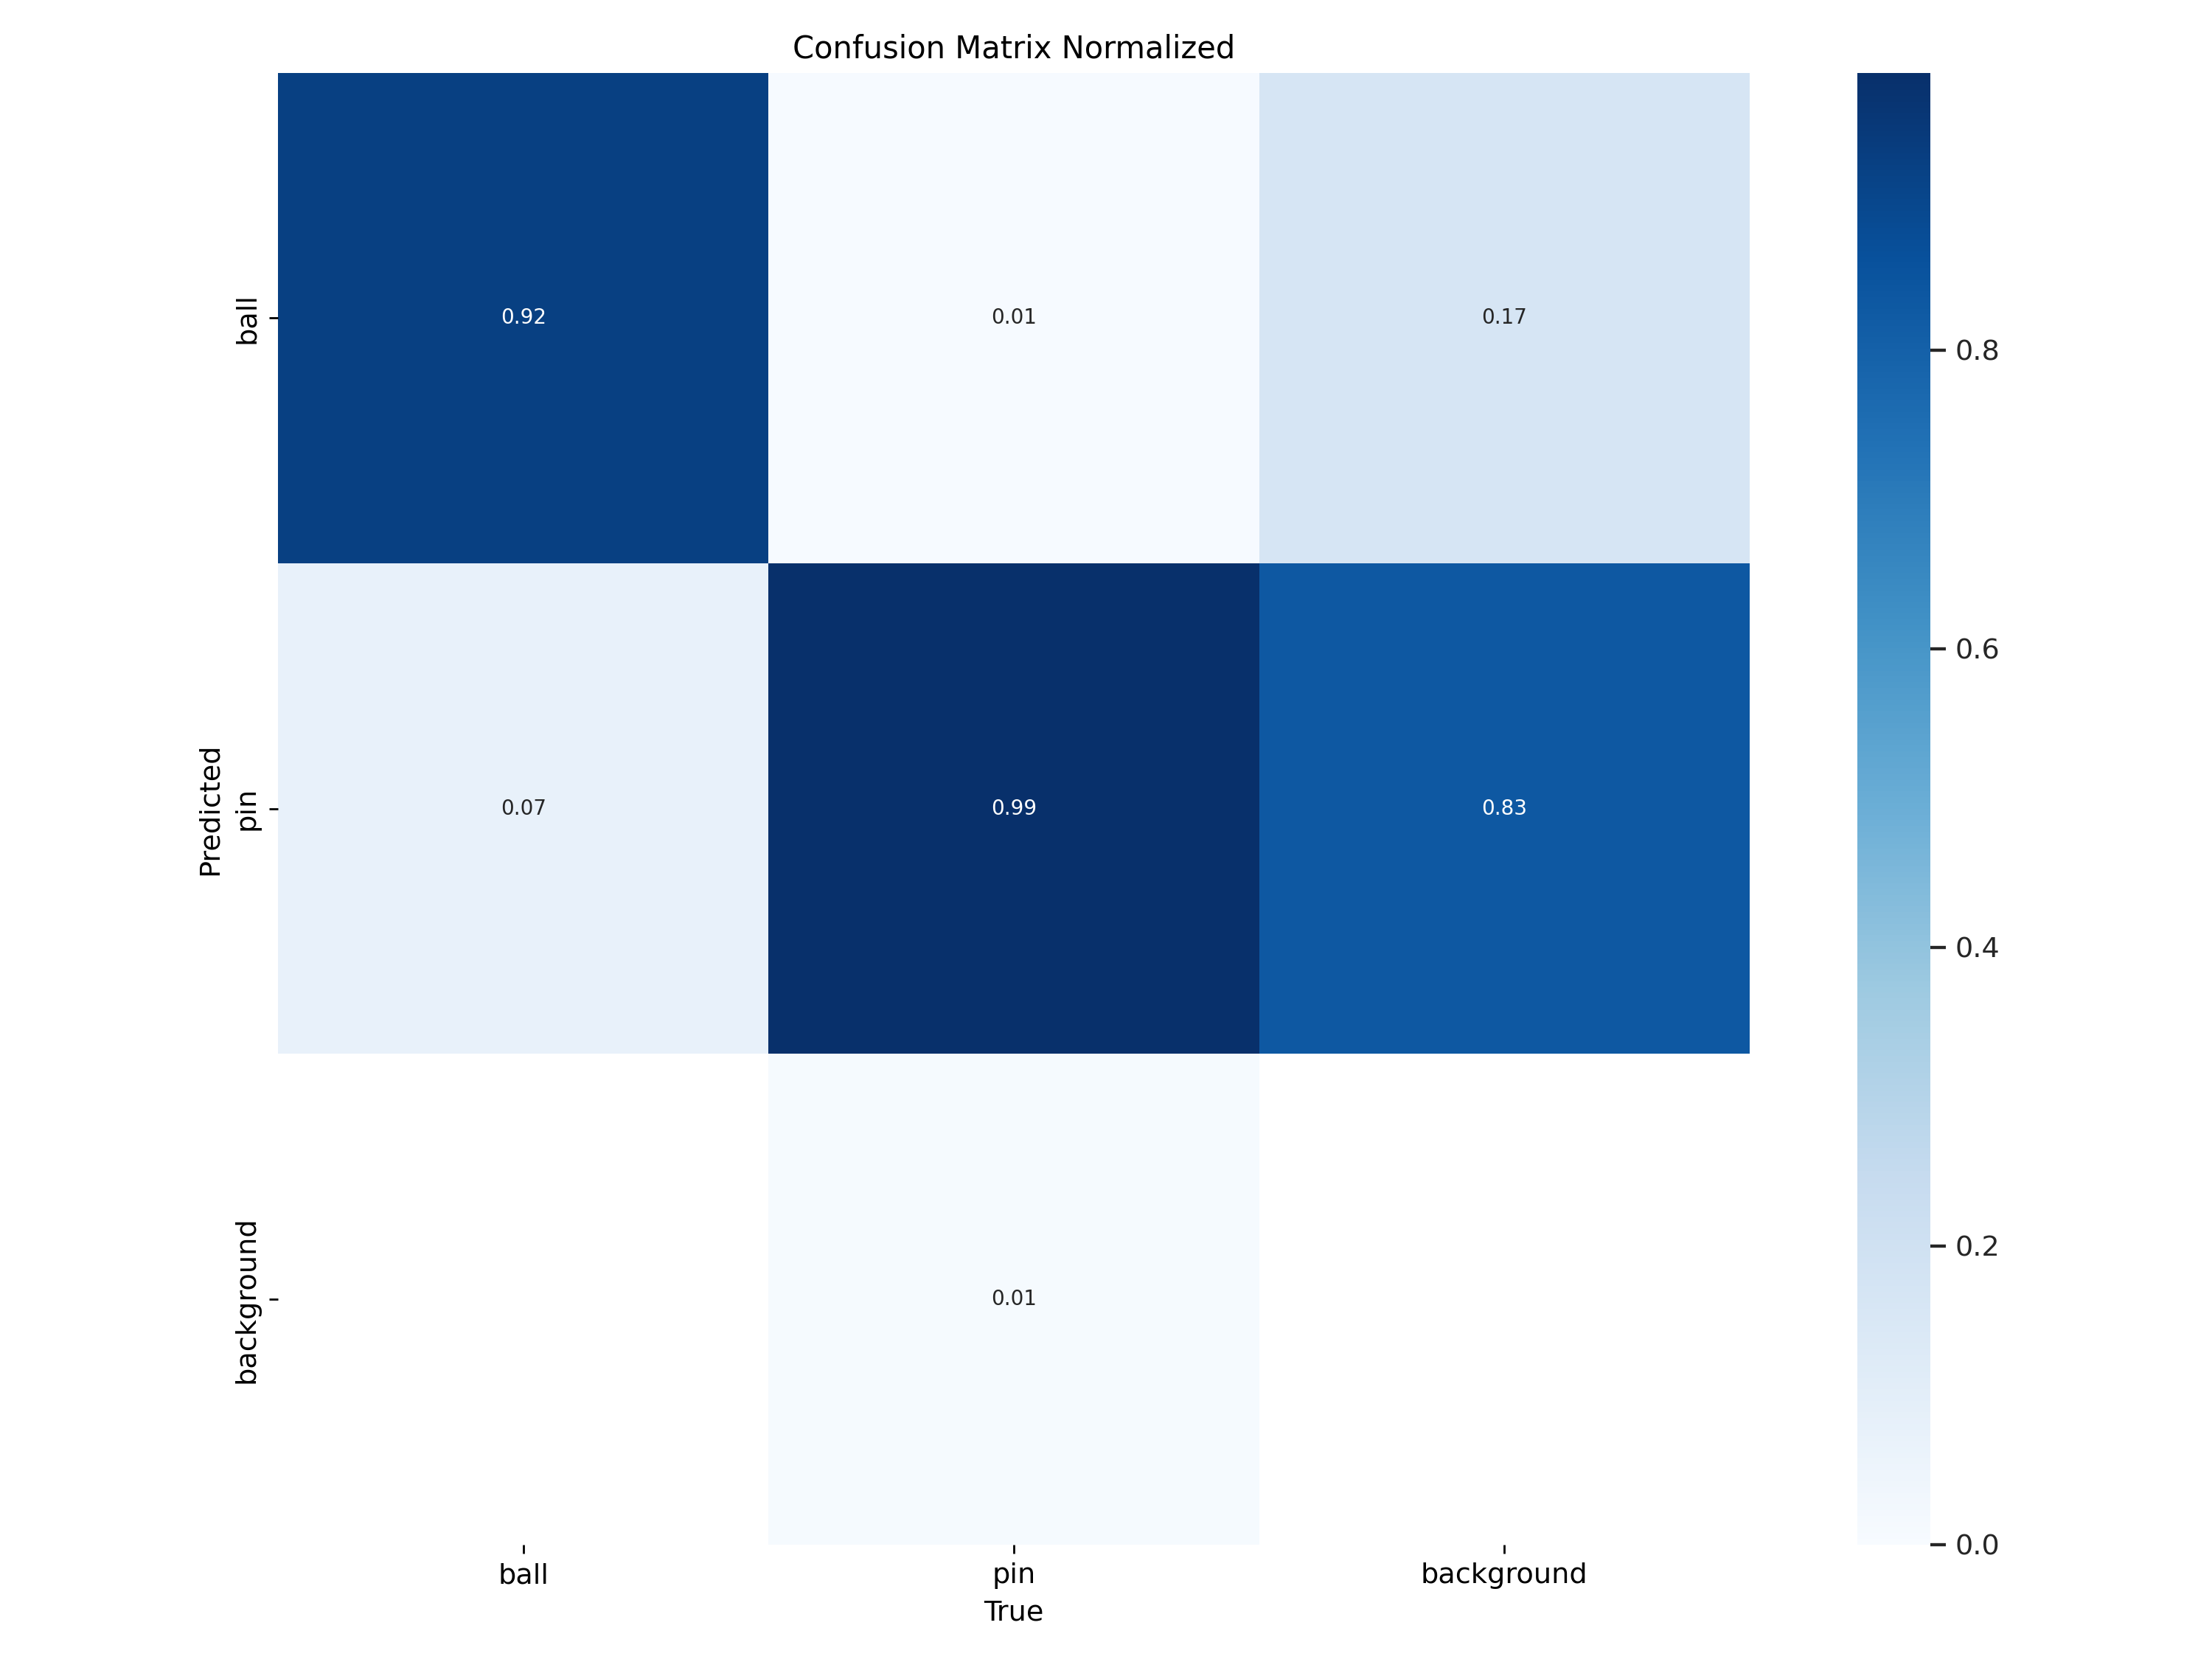
\includegraphics[width=\linewidth]{figures/confusion_matrix_normalized.png}
      \small Normalised confusion matrix (val set)\\
      High diagonal weight for both classes.
    \end{column}
    \begin{column}{0.49\textwidth}
      \centering
      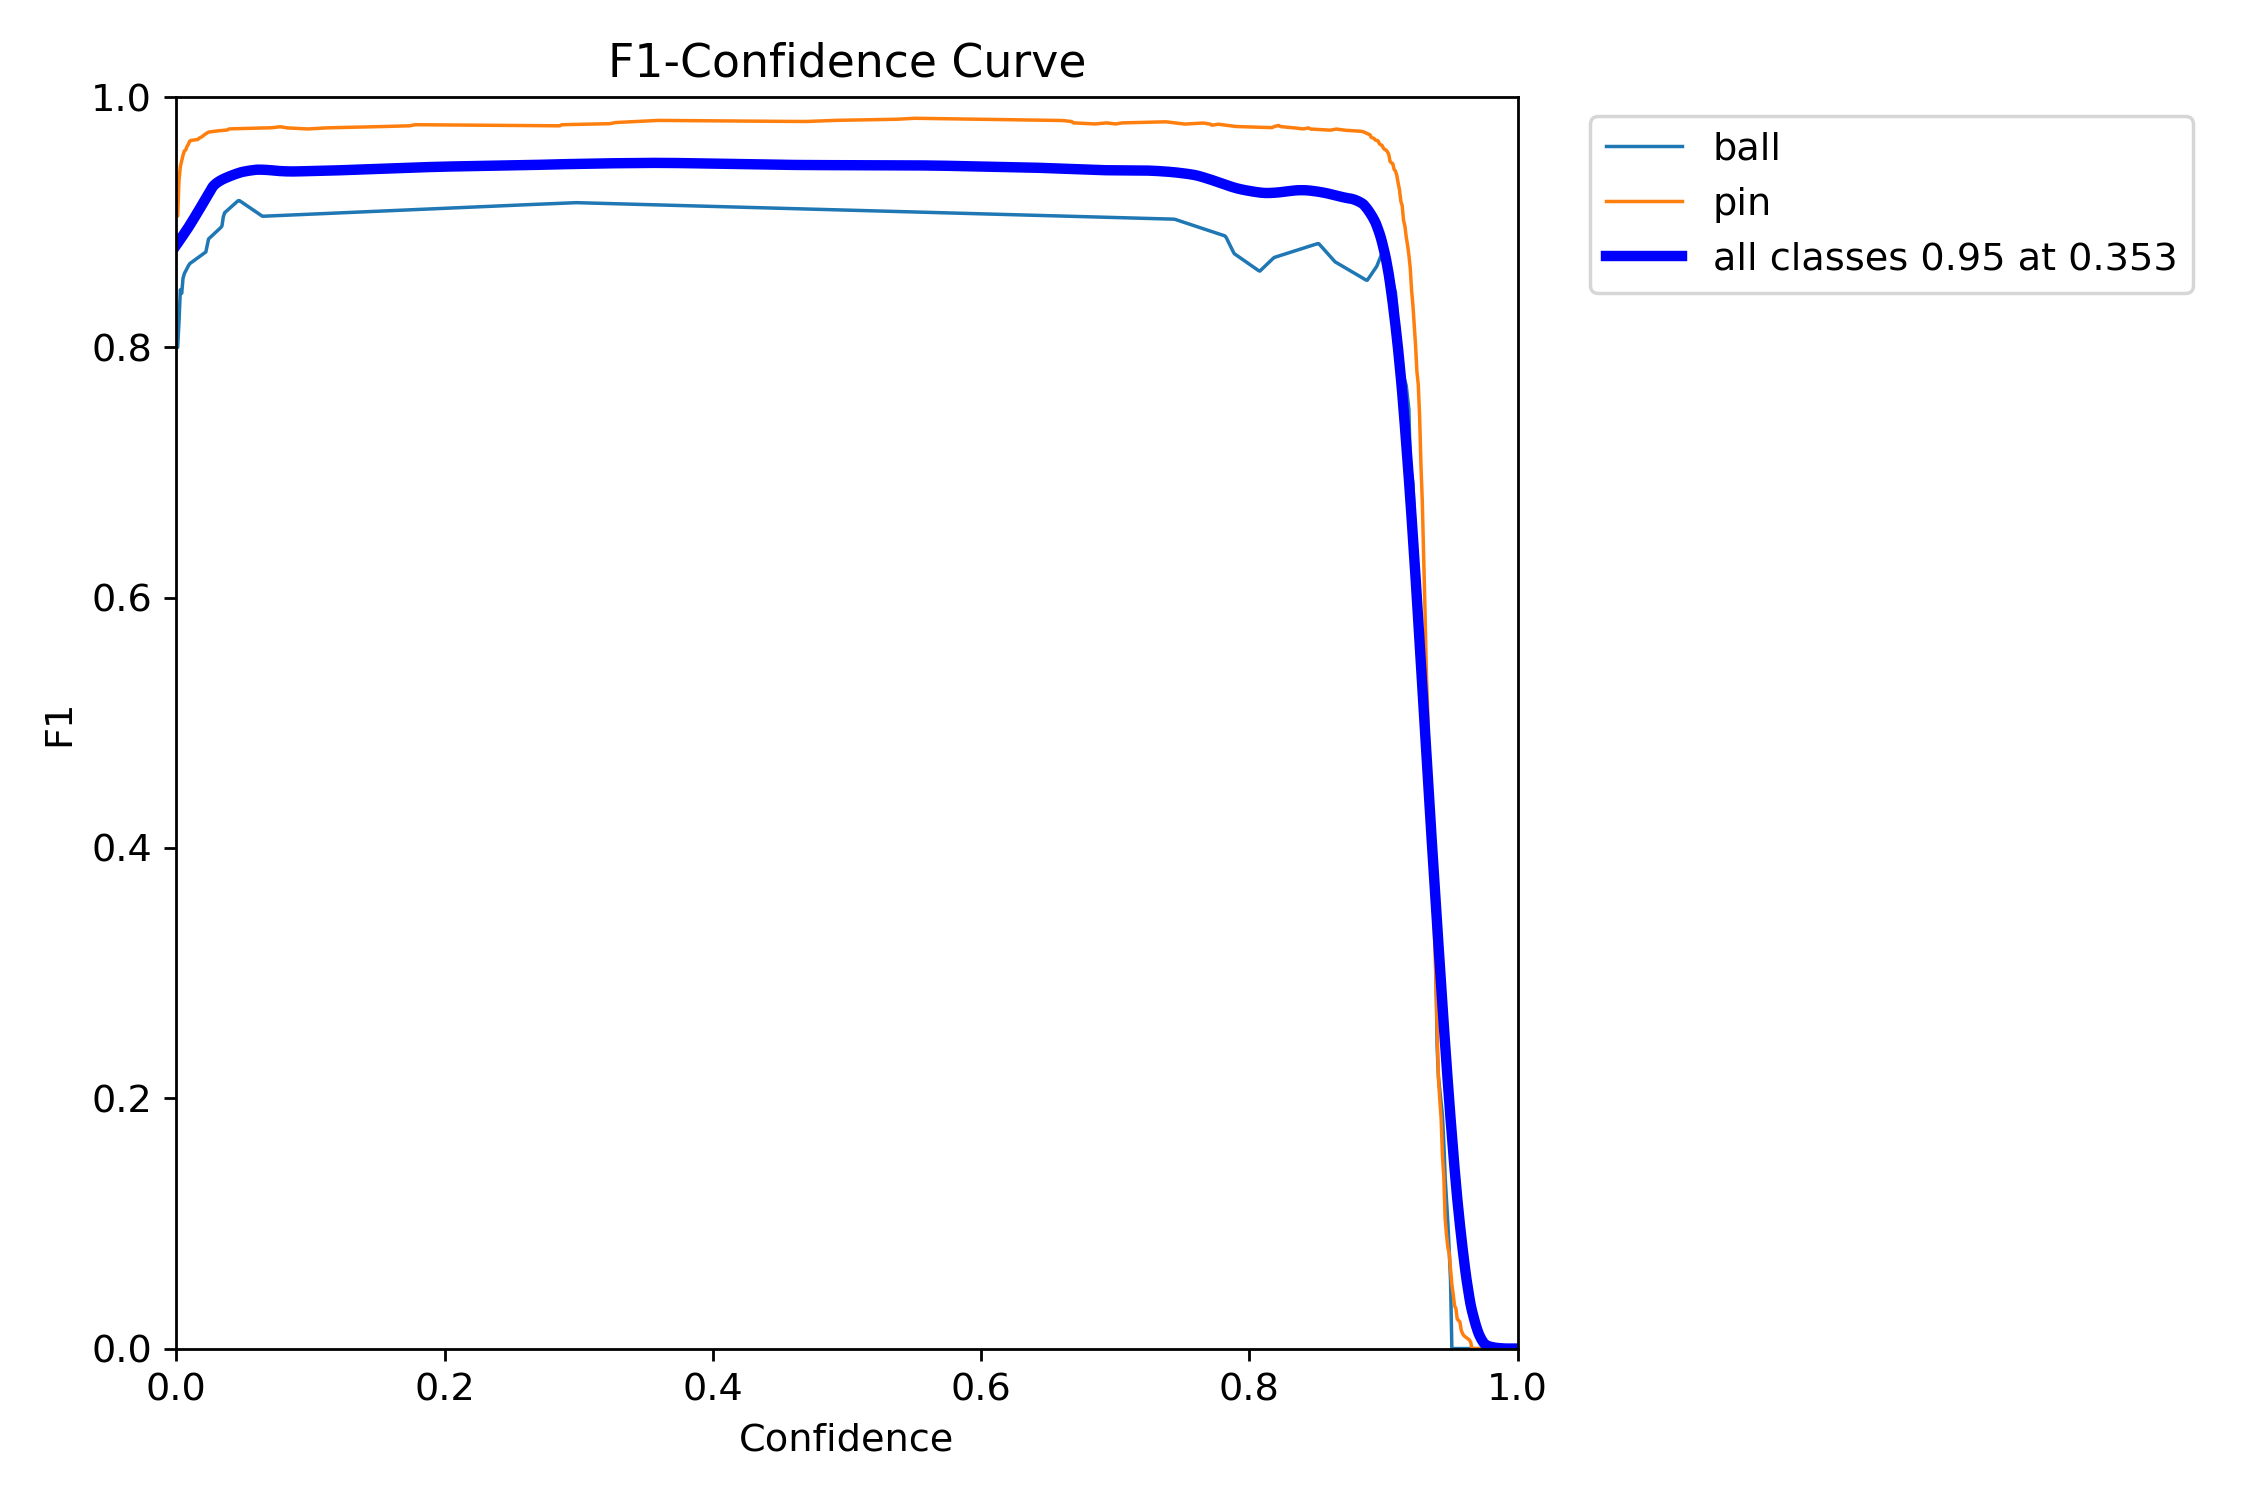
\includegraphics[width=\linewidth]{figures/F1_curve.png}
      \small F1 vs.\ confidence threshold\\
      Flat plateau from conf = 0.10 to 0.30.
    \end{column}
  \end{columns}
\end{frame}

%% ============================================================
%% Slide 13 — Known Limitations
%% ============================================================
\begin{frame}{Known Limitations}
  \begin{enumerate}
    \item \textbf{Axial falls.} Pins falling toward/away from the camera change aspect ratio less. The centroid-drop signal compensates but is weaker; detection may lag by more frames.

    \item \textbf{Tracker ID switches at impact.} Heavy occlusion during ball contact can cause ByteTrack to assign a new ID. The persistent marker then attaches to the new ID rather than the original.

    \item \textbf{Motion blur on the fall frame.} 2--3 frames of blur degrade bounding box shape. The 5-frame sustain threshold mitigates single-frame noise at the cost of a small detection lag.

    \item \textbf{Ball-gate bypass.} If the ball detector fails for $>$60 consecutive frames, the proximity gate is lifted and spurious falls can be triggered.

    \item \textbf{Single-environment dataset.} All 15 clips were recorded in one room. Performance on different backgrounds, lighting, or camera angles is untested.
  \end{enumerate}
\end{frame}

%% ============================================================
%% Slide 14 — Conclusion + Q&A
%% ============================================================
\begin{frame}{Conclusion}
  \begin{itemize}
    \item The fine-tuned YOLOv8s detector achieves \textbf{mAP@50 = 98.19\% (val) / 97.19\% (test)}, meeting and exceeding the accuracy target on both splits.

    \item The full pipeline --- YOLOv8s + ByteTrack + 3-state fall machine + OpenCV renderer --- produces the specified annotated output video with per-pin markers, MM:SS timestamps, HUD, and final summary.

    \item Five failure modes are documented; single-environment training data is the primary robustness bottleneck. Collecting multi-location data is the direct path to improvement.
  \end{itemize}

  \vspace{1.5em}
  \begin{center}
    \Large\textbf{Questions?}
  \end{center}
\end{frame}

\end{document}
